% This sample file is dedicated to the public domain.
\documentclass[12pt]{myucthesis}

%\nofiles
% The above command prevents latex from writing its auxiliary
% files. This is useful if you want to manually tweak them before you
% generate your final PDF.


% Page layout. The fancyhdr package may complain about the need for a
% larger headheight, depending on how long chapter titles are; if left
% unspecified in the geometry setup, it defaults to 12pt. The
% "showframe" option causes the geometry package (version >= 5.0) to
% show a frame around the margins on every page, which is great for
% checking that you don't overflow anywhere.

%\usepackage[letterpaper,includehead,margin=1in,headheight=15pt,showframe]{geometry}
\usepackage[letterpaper,includehead,margin=1in,headheight=15pt]{geometry}
\usepackage{fancyhdr}
\pagestyle{fancyplain}
\lhead[\fancyplain{\thepage}{\thepage}]{\fancyplain{}{\scshape\rightmark}}
\rhead[\fancyplain{}{\scshape\leftmark}]{\fancyplain{\thepage}{\thepage}}
\chead{}
\cfoot{}
\lfoot{}
\rfoot{}


% Bibliography stuff:

\newcommand{\newblock}{\par} % need this for some natbib internal bug
\usepackage{natbib}
\citestyle{cell}
\bibliographystyle{plainnat_robyn}
\setlength{\bibsep}{1ex} % single-space entries
\renewcommand{\bibname}{References}
\def\bibpreamble{\addcontentsline{toc}{chapter}{Bibliography}} % get a good TOC entry


% Other setup:

\usepackage[T1]{fontenc} % see http://tinyurl.com/67zdxwf
\usepackage[colorlinks,urlcolor=blue,citecolor=blue,linkcolor=blue,pdfusetitle]{hyperref}
\usepackage{pdflscape} % allows landscape-oriented figures with PDF page rotation
\usepackage{aasmacros,amsmath,amssymb,graphicx}
\usepackage{mydeluxetable} % deluxetable customized to play well with ucthesis

% MY setup:
\graphicspath{ {figures/}{figures/Chap1/}{figures/Chap2/}{figures/Chap3/}{figures/Chap4/}{figures/Misc/} }  % Location of the graphics files (set up for graphics to be in PDF format)
\usepackage{subfigure}
\usepackage[labelfont=bf,singlelinecheck=off]{caption}
\usepackage[Sonny]{fncychap}
\ChTitleVar{\centering\Large\rm\bfseries}
\usepackage{float}
\usepackage{booktabs}
\usepackage{array}
\newcolumntype{C}[1]{>{\centering\let\newline\\\arraybackslash\hspace{0pt}}m{#1}}
\renewcommand{\tabcolsep}{4pt}
\newcommand{\ra}[1]{\renewcommand{\arraystretch}{#1}}
\renewcommand*{\thesubfigure}{\alph{subfigure}}


\begin{document}
\ssp % single spacing
\hypersetup{pageanchor=false}
\title{Reconstitution of partially recombinant 26S proteasome reveals functional asymmetries in its heterohexameric AAA+ unfoldase}
\author{Robyn Jeanne Beckwith} % must match BearFacts!
\degreesemester{Spring}
\degreeyear{2014}
\degree{Doctor of Philosophy}
\numberofmembers{3}
\chair{Professor Andreas Martin}
\othermembers{
Professor John Kuriyan \\
Professor David Wemmer \\
Professor James Berger
}
\field{Molecular and Cell Biology}
\campus{Berkeley}
\maketitle
\copyrightpage

\begin{abstract}
The 26S proteasome is the major eukaryotic ATP-dependent protease, yet the detailed mechanisms utilized by the proteasomal heterohexameric AAA+ unfoldase to drive sub- strate degradation remain poorly understood. To perform systematic mutational analyses of individual ATPase subunits, we heterologously expressed unfoldase subcomplex from Saccharomyces cerevisiae in Escherichia coli and reconstituted the proteasome in vitro. Our studies demonstrate that the six ATPases play distinct roles in degradation, corresponding to their positions in spiral staircases adopted by the AAA+ domains in the absence and presence of substrate. ATP hydrolysis in subunits at the top of the staircases is critical for substrate engagement and translocation. While the unfoldase relies on this vertical asymmetry for substrate processing, interaction with the peptidase exhibits three-fold symmetry with contributions from every other subunit. These diverse functional asymmetries highlight how the 26S proteasome deviates from simpler, homomeric AAA+ proteases. \\
\\
MORE\ldots My work is awesome. Give me a Ph.D.
\end{abstract}

\hypersetup{pageanchor=true}
\begin{frontmatter}

\pagestyle{plain} 
\begin{dedication}
\null\vfil
{\large
\begin{center}
I dedicate this dissertation to graduate students everywhere.
\end{center}}
\null\vfil
\end{dedication}

\tableofcontents
\addcontentsline{toc}{chapter}{Table of Contents}
\listoffigures % optional
\listoftables % optional

% If using code.sty, can also add:
%% \listofcodes
%% \addcontentsline{toc}{chapter}{List of Code Examples}

\begin{acknowledgements}
Stuff.

% Feel free to modify or remove this acknowledgment:
%This dissertation was typeset using the
%\href{https://github.com/pkgw/ucastrothesis}{\textsf{ucastrothesis}}
%\LaTeX\ template.

\end{acknowledgements}
\end{frontmatter}


% Chapter 1

\chapter{Introduction} % Write in your own chapter title
\label{Chapter1}
\lhead{Chapter 1. \emph{Introduction}} % Write in your own chapter title to set the page header


\section{The cellular roles and common architecture of ATP-dependent proteases}

Proteins are an integral component of cells responsible for structural organization, signaling and carrying out chemical reactions required to sustain life.  The specific lifetime of a given protein plays a critical role in its function and protein degradation is required for modulating regulatory proteins as well as maintaing protein quality control.  (PROCESSES) In all cells, selective protein destruction is a tightly regulated process mediated by energy-dependent proteases.  

The specificity of protein degradation by these molecular machines is achieved through a common architecture of a barrel-shaped peptidase capped by a protein unfoldase ring.  The promiscuous proteolytic active sites of the peptidase are sequestered inside a barrel-shaped chamber formed by stacked oligomeric rings.  Substrate entry to the degradation chamber is restricted by the narrow axial pores of the peptidase and must be facilitated by a ring of AAA+ (\textit{A}TPases \textit{A}ssociated with various cellular \textit{A}captivities) proteins that sits atop the peptidase.

%protease figure

%%-------------------------
\begin{figure}[b!]
\centering
\setlength{\fboxrule}{0pt}
\fbox{%
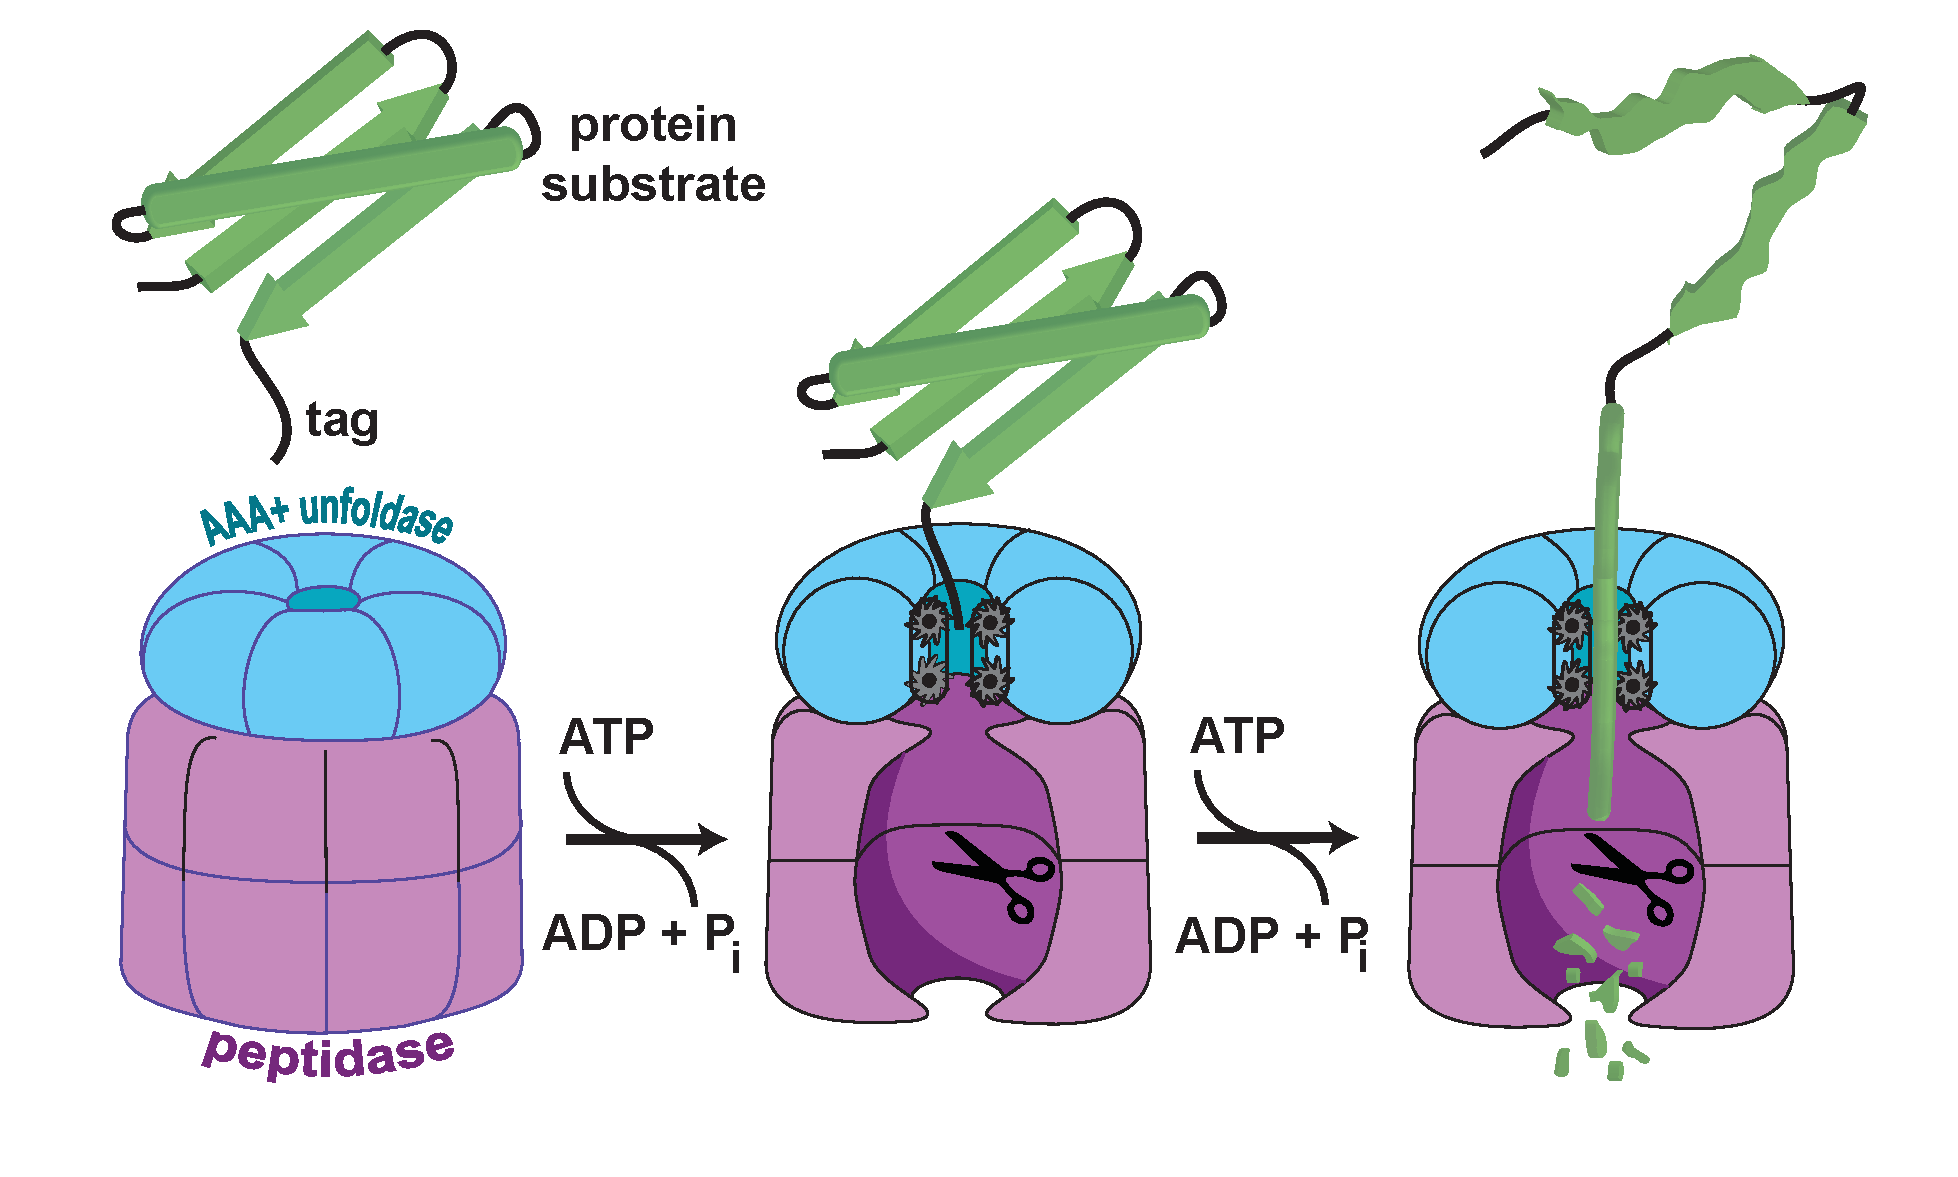
\includegraphics[scale=.4]{protease_robyn}% 
}
\caption[title]{title.\par
Adapted from ~\citet{Nyquist2014}. 
}
\label{fig:wbsto}
\end{figure}
%%-------------------------



CP active sites

large and small AAA+ domains, coordinated ATP hydrolysis

central pore, pore loops
power strokes
subunit communication
interface of unfoldase and peptidase



prokaryotic vs eukaryotic

\section{26S proteasome structure and assembly}
%EM 26S structure and subcomplexes
%base subunit architecture, EM structure and subunit schematic
%assembly

core
lid
base
chaperones
tails

complexity

\section{Steps in substrate processing}
%derivative of mary's schematic
ubiquitin binding
engagement
translocation and unfolding
deubiquitination - ubiqitin recycling
degradation - peptide release

ubiquitin chain linkage/length - affinity, binding orientation
substrate geometry - engagement
substrate stability - translocaton and unfolding 

how does heterohexameric architecture contribute to added complexity


\

\section{AAA+ protein unfoldases}
%active site
% top view with pore loops (pan or clpx?)
%rpt seq alignment (or put in main text as data?)

conserved AAA+ motifs
catalytic cycle
rigid body
pore loops
interaction with peptidase

\section{Subunit specialization in the heterohexameric AAA+ unfoldase of the proteasome}
	In this dissertation, we explore how the six distinct ATPase subunits of the proteasomal unfoldase are involved in substrate processing, interaction with the core peptidase and coordinated ATP hydrolysis.  To accomplish unprecedented systematic \textit{in vitro} studies, we developed a heterologous expression system to produce the unfoldase subcomplex from \textit{S. cerevisieae} in \textit{E. coli} and established conditions to reconstitute partially recombinant 26S proteasomes (Chapter~\ref{Chapter2}).\par
	Detailed analysis of the individual roles of the six proteasomal ATPase subunits in substrate processing required the biochemical characterization of catalytic mutations in conserved AAA+ motifs.  A mutation in the canonical AAA+ Walker\--B motif was used to trap single subunits in a defined ATP-bound state in order to define the contributions of individual subunits to substrate processing.  We demonstrate that the six ATPase subunits are functionally distinct and that ATP hydrolysis by Rpt3, Rpt4 and Rpt6 is crucial for successful substrate degradation.  These subunits are located at the top of the spiral staircase configuration of ATPases observed in the proteasomal unfoldase in absence of substrate, indicating that ATP hydrolysis may these subunits is potentially required for substrate engagement. (TRANSITION) We examined the importance of individual ATPase subunits for base-core association and demonstrated that peptidase binding and gate opening do not depend on the nucleotide state of specific Rpt C-terminal tails (Chapter~\ref{Chapter3}).\par
	Pursuant to these studies we explored the coordination of ATP hydrolysis within the base ATPase ring by  mutating the arginine finger to disrupt communication between neighboring subunits.  We further developed a series of concatamer substrates to deconvolute the processes of substrate engagement verses translocation by the proteasome base.  This tool will facilitate a more mechanistic understanding of how various mutants compromise substrate processing by the proteasome (Chapter~\ref{Chapter4}).\par
	Prior to these studies we lacked an understanding of how the heterohexameric architecture of the base unfoldase affects proteasomal substrate processing or subcomplex interactions.  Our work provides systematic and quantitative insights into the specialization of ATPase subunits in various aspects of proteasome function, including substrate engagement and translocation, interaction with the core peptidase, and the coordination of ATP hydrolysis.\par
	


% Chapter 2

\chapter{Heterologous expression of the base unfoldase} % Write in your own chapter title
\label{Chapter2}
\lhead{Chapter 2. \emph{Heterologous expression of the base unfoldase}} % Write in your own chapter title to set the page header


\section{Introduction}
Previous work investigating proteasome function has been complicated by the fact that cell viability is strictly dependent on proteasome function. The essential nature of the proteasome has additionally limited mutational studies both \textit{in vivo} and \textit{in vitro}, largely preventing systematic analyses of the mechanisms of proteasomal protein degradation and subcomplex interactions. Furthermore, isolation of proteasome holoenzyme or subcomplexes has been limited by low sample yields and significant subunit heterogeneity. Heterologous expression of the base subcomplex circumvents these issues by generating high yields of base with defined subunit composition that can be mutated or altered without affecting bacterial cell viability. To facilitate detailed mechanistic studies of the proteasomal unfoldase, we therefore designed a system for the expression of the base subcomplex from \textit{Saccharomyces cerevisiae} in \textit{Escherichia coli}. 


%%-------------------------

\section{Results}

\subsection{Cloning, expression and purification of recombinant base}

The base subcomplex of the proteasome from \textit{Saccharomyces cerevisiae} was produced in \textit{Escherichia coli} by co-expression of thirteen yeast proteins, including nine integral base subunits (Rpt1\--6, Rpn1, Rpn2, Rpn13) and four proteasome assembly chaperones (Nas2, Nas6, Rpn14, Hsm3~\citep{Funakoshi2009,Roelofs2009,Saeki2009,Kaneko2009}) as depicted in Figure \ref{fig:vectors}. We isolated assembled base by tandem-affinity purification using tags on two different subunits, followed by gel\--filtration chromatography (Figure \ref{fig:sizing}). The purified base exhibited appropriate stoichiometry and no subunit truncations, as revealed by SDS\---PAGE (Figure \ref{fig:basegel}) and mass spectrometry (data not shown, R.B.). We observed Nas6, Hsm3, and Rpn14 stably associated with the recombinant base, whereas these chaperones were not present in the base purified from yeast, as indicated by SDS\--PAGE, size\--exclusion chromatography, and native PAGE (Figure \ref{fig:nativegel}).

%----------------------------- 

\begin{figure}[t]
\centering
\setlength{\fboxrule}{0pt}
\fbox{%
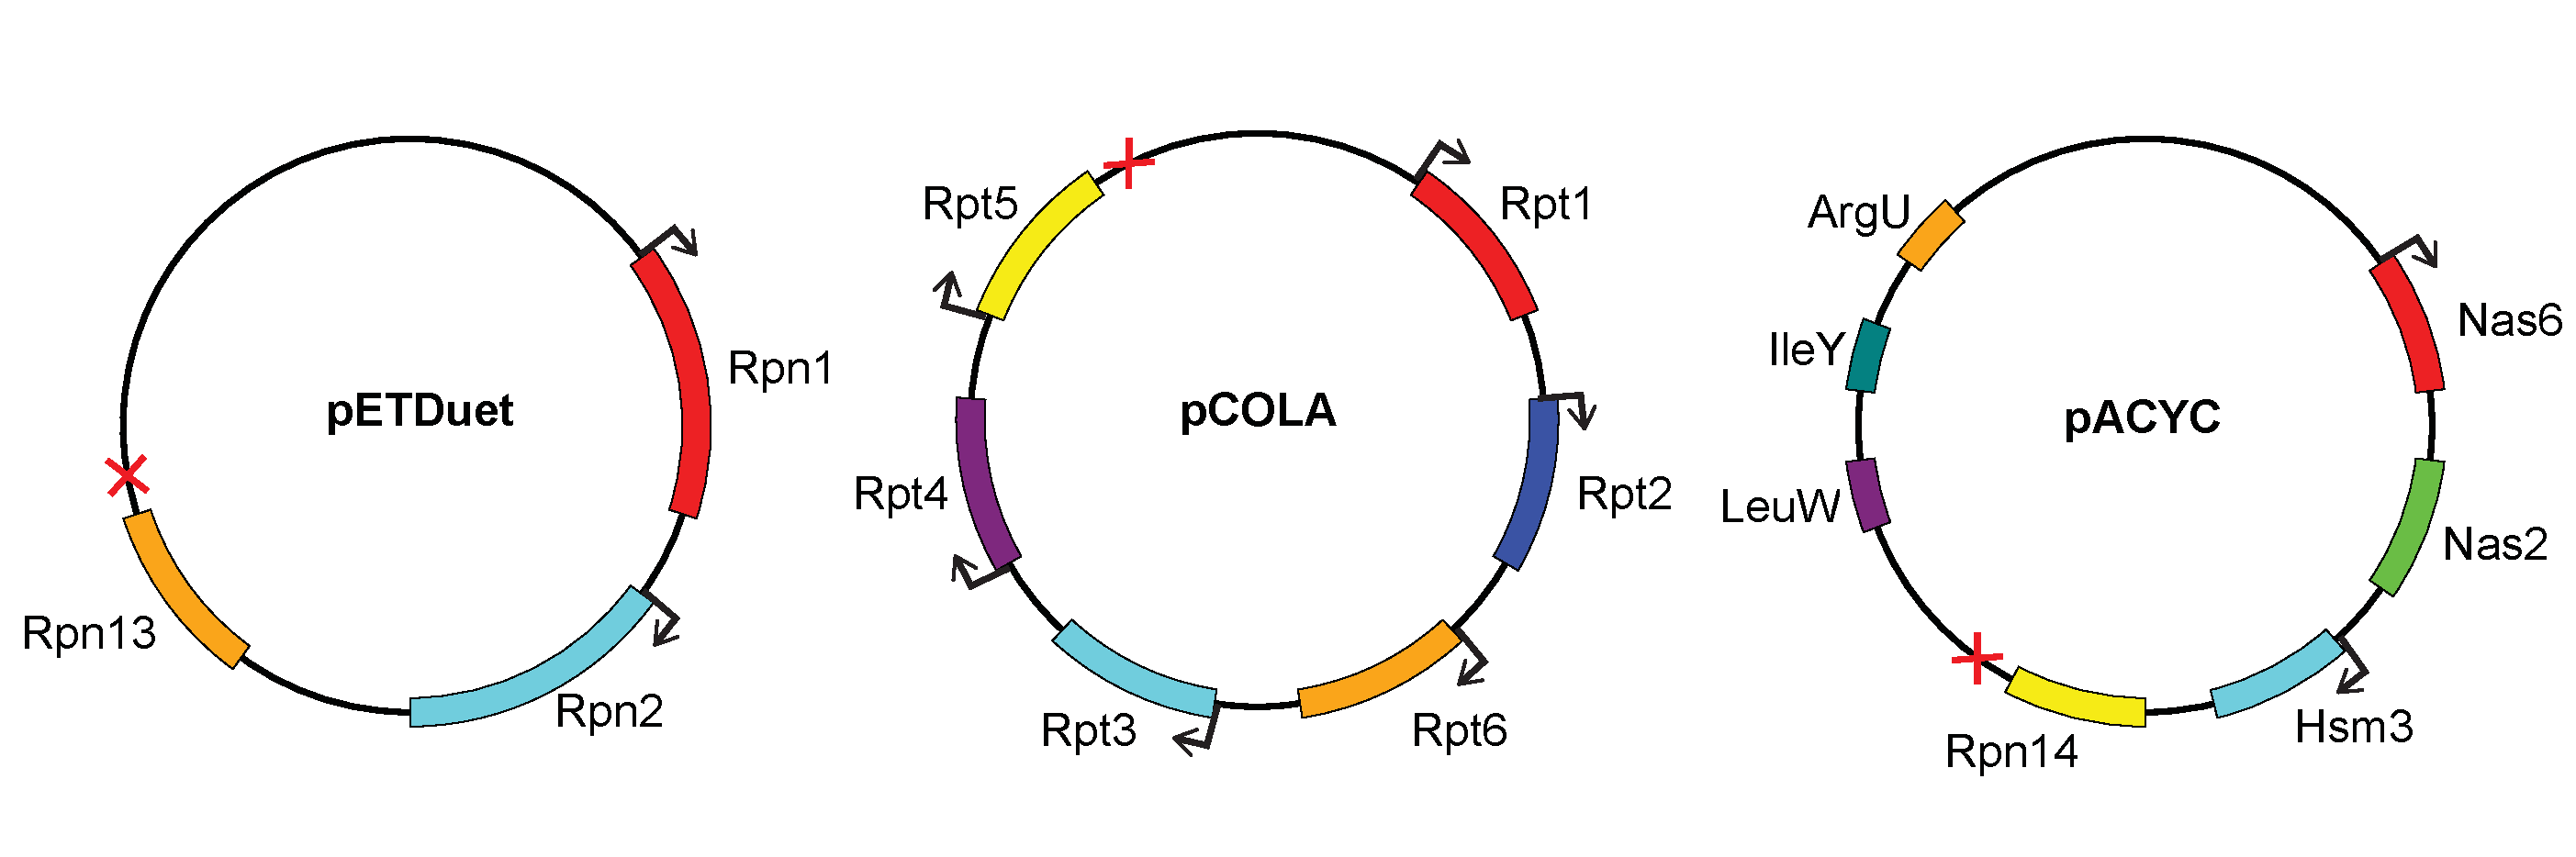
\includegraphics[scale=0.32]{vectors}%
}
\caption[Plasmid maps for recombinant base expression]{Plasmid maps for recombinant base expression.\par
The base subcomplex from \textit{S. cerevisiae} was heterologously produced in \textit{E. coli} by co-expression of thirteen proteins encoded on three plasmids with different antibiotic resistances. pETDuet (Amp$^{res}$) contained three non-ATPase subunits of the base, while the six distinct ATPases were encoded by pCOLA (Kan$^{res}$). Base production required co\--expression with four base\--specific proteasome chaperones that were included on pACYC (Chl$^{res}$), which also contained genes for rare tRNAs.
}
\label{fig:vectors}
\end{figure}

%-----------------------------

\begin{figure}[h!]
\centering
\subfigure{%
	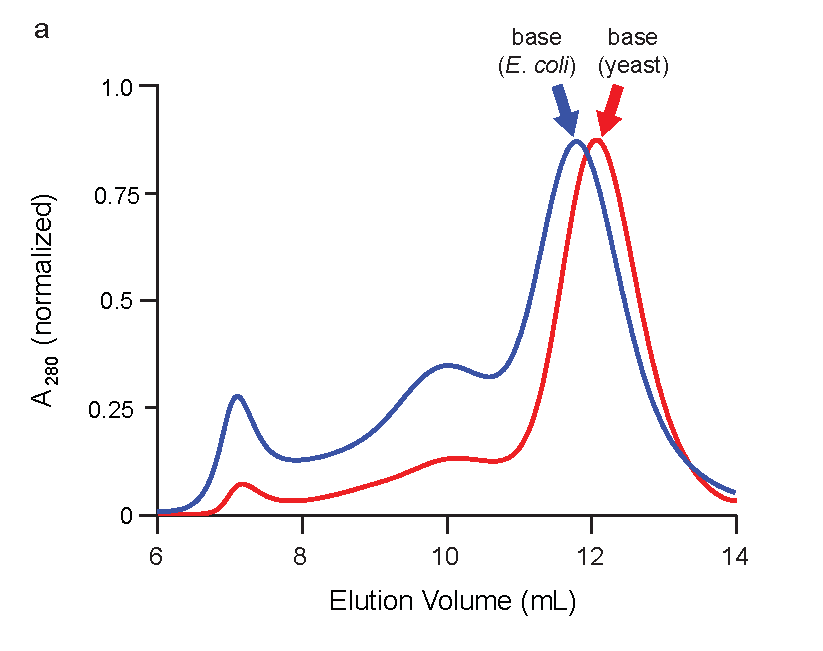
\includegraphics[scale=0.6]{sizing}
	\label{fig:sizing}}
\quad	
\subfigure{%
	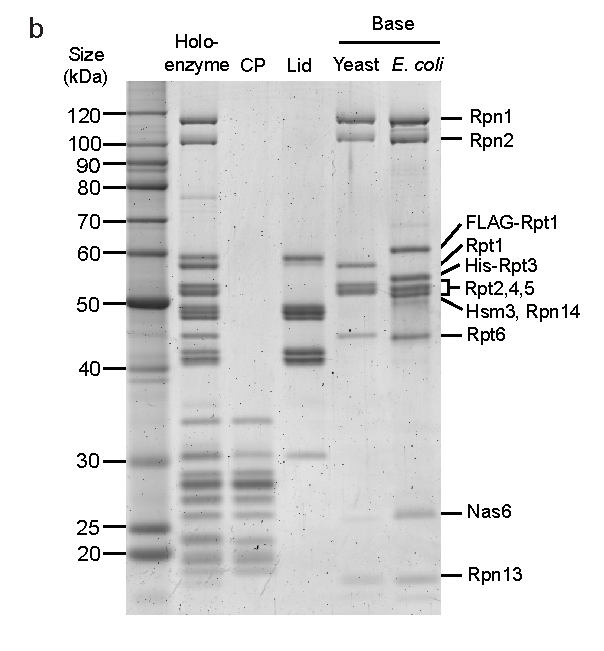
\includegraphics[scale=0.6]{basegel}
	\label{fig:basegel}}
%
\caption[Purification of the recombinant base and yeast proteasome subcomplexes]{Purification of the recombinant base and yeast proteasome subcomplexes.\par
\textbf{(a)} Endogenous (red) and \textit{E. coli}\--expressed, recombinant (blue) base subcomplexes show similar elution profiles from a Superose 6 size\--exclusion column. The slightly smaller elution volume for recombinant base is attributed to the co-purification of proteasome\--specific chaperones that stably associate with the complex when heterologously expressed in the absence of core particle in \textit{E. coli}. The absorbance at 280 nm is normalized for comparison. For equal cell mass, recombinant base expression yields approximately 10\--fold more protein than the purification of endogenous base from yeast. \textbf{(b)} Sypro\--Ruby stained SDS\--PAGE of the purified proteasomal subcomplexes used in this study. Endogenous complexes were isolated from yeast using FLAG tags on Rpn11 for holoenzyme and lid, on Pre1 for core particle (CP), and on Rpn2 for base preparations. Recombinant base expressed in \textit{E. coli} was purified using a FLAG tag on Rpt1 and a His$_6$ tag on Rpt3. Proteasome chaperones Nas6, Hsm3 and Rpn14 only co\--purify with the base subcomplex produced in \textit{E. coli}.
}
\label{fig:basesizing}
\end{figure}

%-----------------------------

This result is consistent with studies of \textit{in\--vivo} proteasome assembly, indicating that Nas6, Hsm3, and Rpn14 are displaced upon base binding to the core particle and lid, whereas Nas2 dissociates at an earlier stage of base assembly~\citep{Funakoshi2009,Roelofs2009,Park2009,Park2013}. One model for \textit{in\--vivo} base assembly proposes that the core particle might act as a template to facilitate the proper arrangement of Rpts in the hexameric ring~\citep{Park2009}. However, our successful production of the base subcomplex in \textit{E. coli} rules out a strict requirement for such templated assembly. \par

We compared the activities of the recombinant base to endogenous yeast base. Both base subcomplexes hydrolyzed approximately 51 ATP enz$^{-1}$ min$^{-1}$ in the absence of substrate (Table~\ref{table:holoenzyme}). The ability of the ATP\--bound base to interact with core particle and induce gate opening was determined by monitoring the fluorescence increase upon peptidase cleavage of the fluorogenic peptide succinyl\--Leu\--Leu\--Val\--Tyr\--(7\--amino\--4\--methylcoumarin). In the presence of ATP, recombinant base stimulated core\--particle activity approximately 20\--fold, similar to endogenous yeast base. In agreement with previous reports, we measured about two-fold higher peptide hydrolysis with the non\--hydrolysable analog ATP$\gamma$S compared to ATP~\citep{Smith2005,Liu2006} which may be due to potential differences in the ATPase\--ring conformation~\citep{Sledz2013} or the dynamics of base\--core interactions. 

%nucleotides?


\subsection{Reconstitution of functional 26S proteasome}

Importantly, we reconstituted 26S holoenzyme using either endogenous or recombinant base and the lid and core particle purified from yeast. Successful reconstitution was assessed by native PAGE (Figure \ref{fig:nativegel}) and \textit{in\--vitro} degradation of a polyubiquitinated model substrate, a green fluorescent protein (GFP)\--titin$^{V15P}$\--cyclin\--PY fusion, whose degradation could be measured through the decrease of GFP fluorescence (Figure \ref{fig:degpanels}, Figure \ref{fig:gfpdeg}). 

Proteasomes reconstituted with saturating recombinant or endogenous base degraded substrate at a maximal rate of 0.3 enz$^{-1}$ min$^{-1}$, comparable to 0.32 enz$^{-1}$ min$^{-1}$ observed for holoenzyme purified from yeast (Table~\ref{table:holoenzyme}). Substrate degradation by reconstituted proteasomes strictly required addition of recombinant Rpn10, an intrinsic ubiquitin\--receptor that does not co\--purify with isolated lid or base subcomplexes. Consistent with previously described degradation defects in the absence of Rpn10~\citep{Verma2004}, we found that omitting Rpn10 or deleting its ubiquitin\--interacting motif resulted in 40\--fold slower degradation (Figure \ref{fig:deg}, Figure \ref{fig:degcontrols}), despite the presence of the second ubiquitin receptor, Rpn13. Since proteasome formation did not depend on Rpn10 (data not shown, R.B.) and degradation was not facilitated by Rpn10 lacking its ubiquitin\--interacting motif, this result suggests that Rpn10 is either the primary receptor for our model substrates or required in combination with Rpn13 for multivalent ubiquitin\--chain binding.

%-----------------------------

\begin{figure}[H]
\centering
\setlength{\fboxrule}{0pt}
\fbox{%
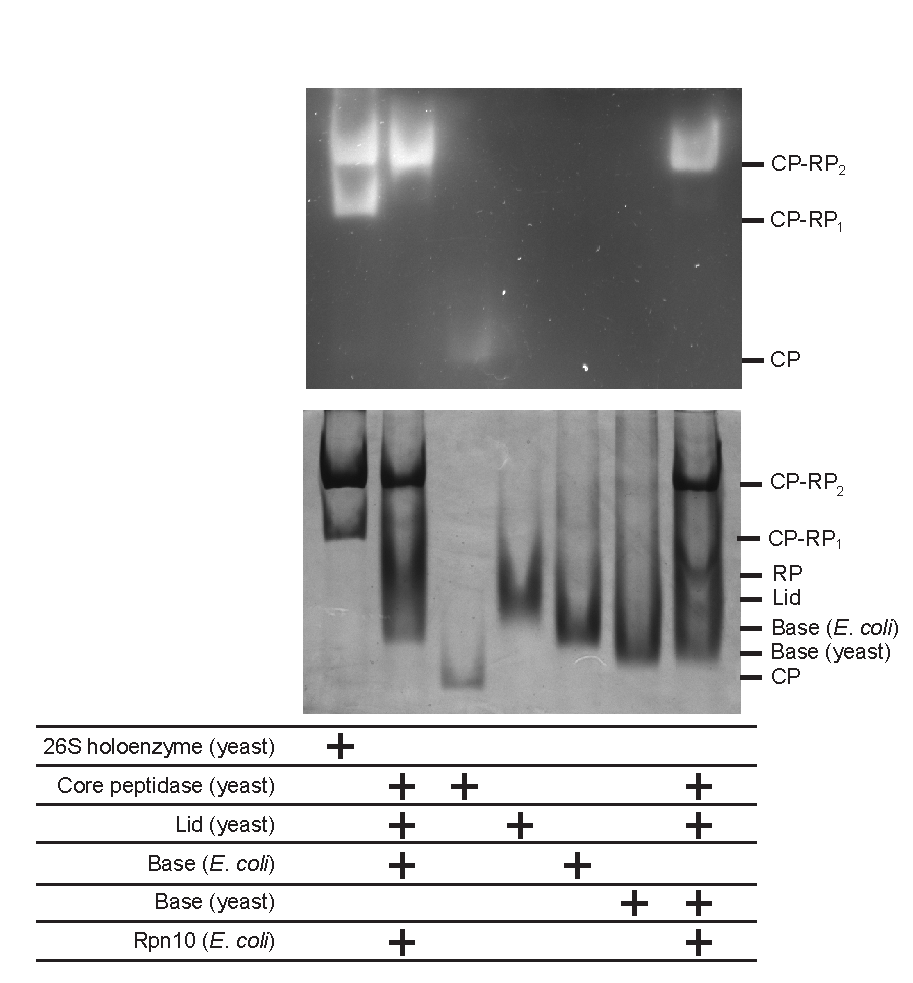
\includegraphics[scale=0.7]{nativegel}% 
}
\caption[Native gel of purified subcomplexes and reconstituted proteasome]{Native gel of purified subcomplexes and reconstituted proteasome.\par
26S holoenzyme reconstituted with CP, lid, Rpn10, and either endogenous or recombinant base was analyzed by native gel electrophoresis. Endogenous yeast 26S holoenzyme and individual CP, lid, and base subcomplexes were also analyzed for comparison. Yeast holoenzyme migrated as two bands corresponding to proteasomes singly (CP\--RP$_1$) and doubly (CP\--RP$_2$) capped with regulatory particles (RP). Excess lid and base was used for reconstituted proteasome samples, which therefore migrated only as doubly capped holoenzyme.}
\label{fig:nativegel}
\end{figure}


%-----------------------------


\begin{table}[H]
\centering
\ra{1.3}
\caption[Biochemical characterization of reconstituted 26 proteasomes]{Biochemical characterization of reconstituted 26 proteasomes.}
\begin{tabular*}{\textwidth}{@{}lcccccccc@{}}\toprule
& \multicolumn{2}{c}{basal ATPase rate} & \phantom{a}& \multicolumn{2}{c}{peptidase stimulation} & 
\phantom{a} & \multicolumn{2}{c}{degradation rate (k$_{deg}$)}\\
\cmidrule{2-3} \cmidrule{5-6} \cmidrule{8-9}
& min$^{\--1}$ & \% WT & & fold increase & \% WT & & (enz$^{\--1}$ min$^{\--1}$) & \% WT\\ \midrule
Holoenzyme & 107 & \--- & & \--- & \--- & & $0.32$ & \---\\
WT (\textit{E. coli}) & 51 & 100 & & 21 & 100 & & 0.30 & 100\\
WT (yeast) & 54 & 106 & & 22 & 103 & & 0.29 & 97\\
\bottomrule
\end{tabular*}
\label{table:holoenzyme}
\end{table}


%-----------------------------
\vfill

\begin{figure}[H]
\centering
\subfigure{%
	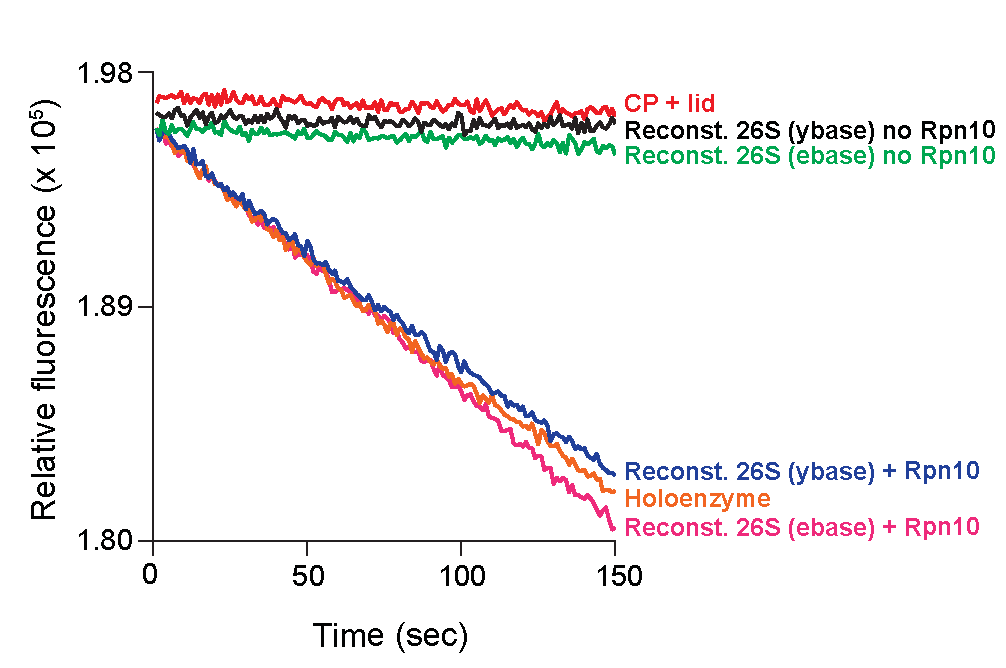
\includegraphics[scale=0.49]{deg}
	\label{fig:deg}}
\quad	
\subfigure{%
	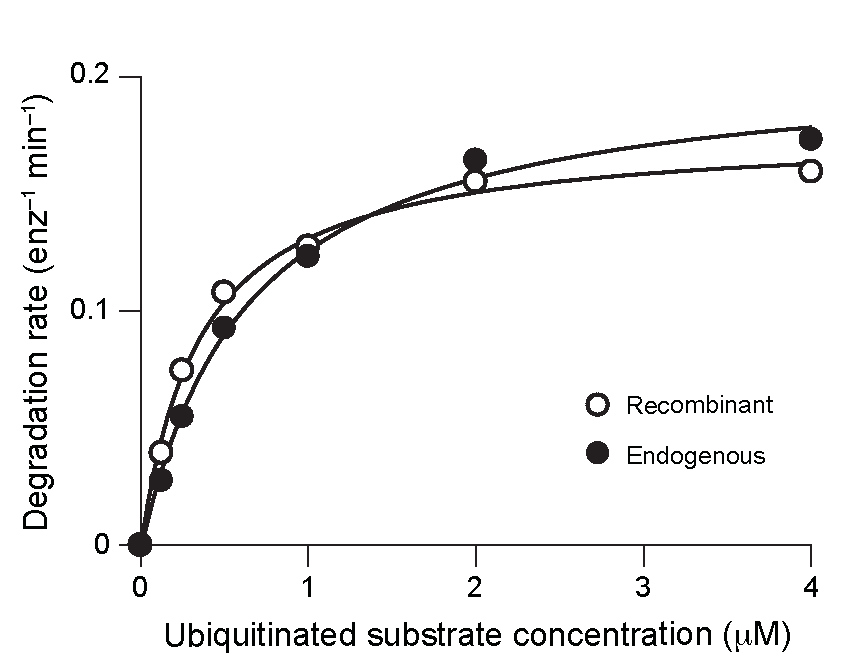
\includegraphics[scale=0.49]{mmdeg}
	\label{fig:mmdeg}}
%
\caption[Degradation of GFP\--fusion substrates by reconstituted proteasomes]{Measuring proteasomal degradation of a ubiquitinated GFP\--fusion substrate.\par
\textbf{(a)} Degradation of a polyubiquitinated GFP fusion substrate by endogenous yeast holoenzyme or 26S proteasomes reconstituted with saturating recombinant base (ebase) or endogenous yeast base (ybase). Substrate degradation was monitored by the loss of GFP fluorescence and strictly required the addition of Rpn10, despite the presence of Rpn13 (see Figure \ref{fig:basegel}). \textbf{(b)} Michaelis\--Menten analyses of substrate degradation by proteasomes reconstituted with endogenous or recombinant base. Degradation reactions were performed using limiting base and excess core particle, lid and Rpn10 to ensure that reconstituted proteasome particles were singly capped. K$_M$ and V$_{max}$ values were 0.63 $\mu$M and 0.21 enz$^{-1}$ min$^{-1}$ for holoenzyme with endogenous base, and 0.35 $\mu$M and 0.18 enz$^{-1}$ min$^{-1}$ for holoenzyme with recombinant base.
}
\label{fig:degpanels}
\end{figure}

%-----------------------------

\newpage
\vfill

\begin{figure}[H]
\centering
\setlength{\fboxrule}{0pt}
\fbox{%
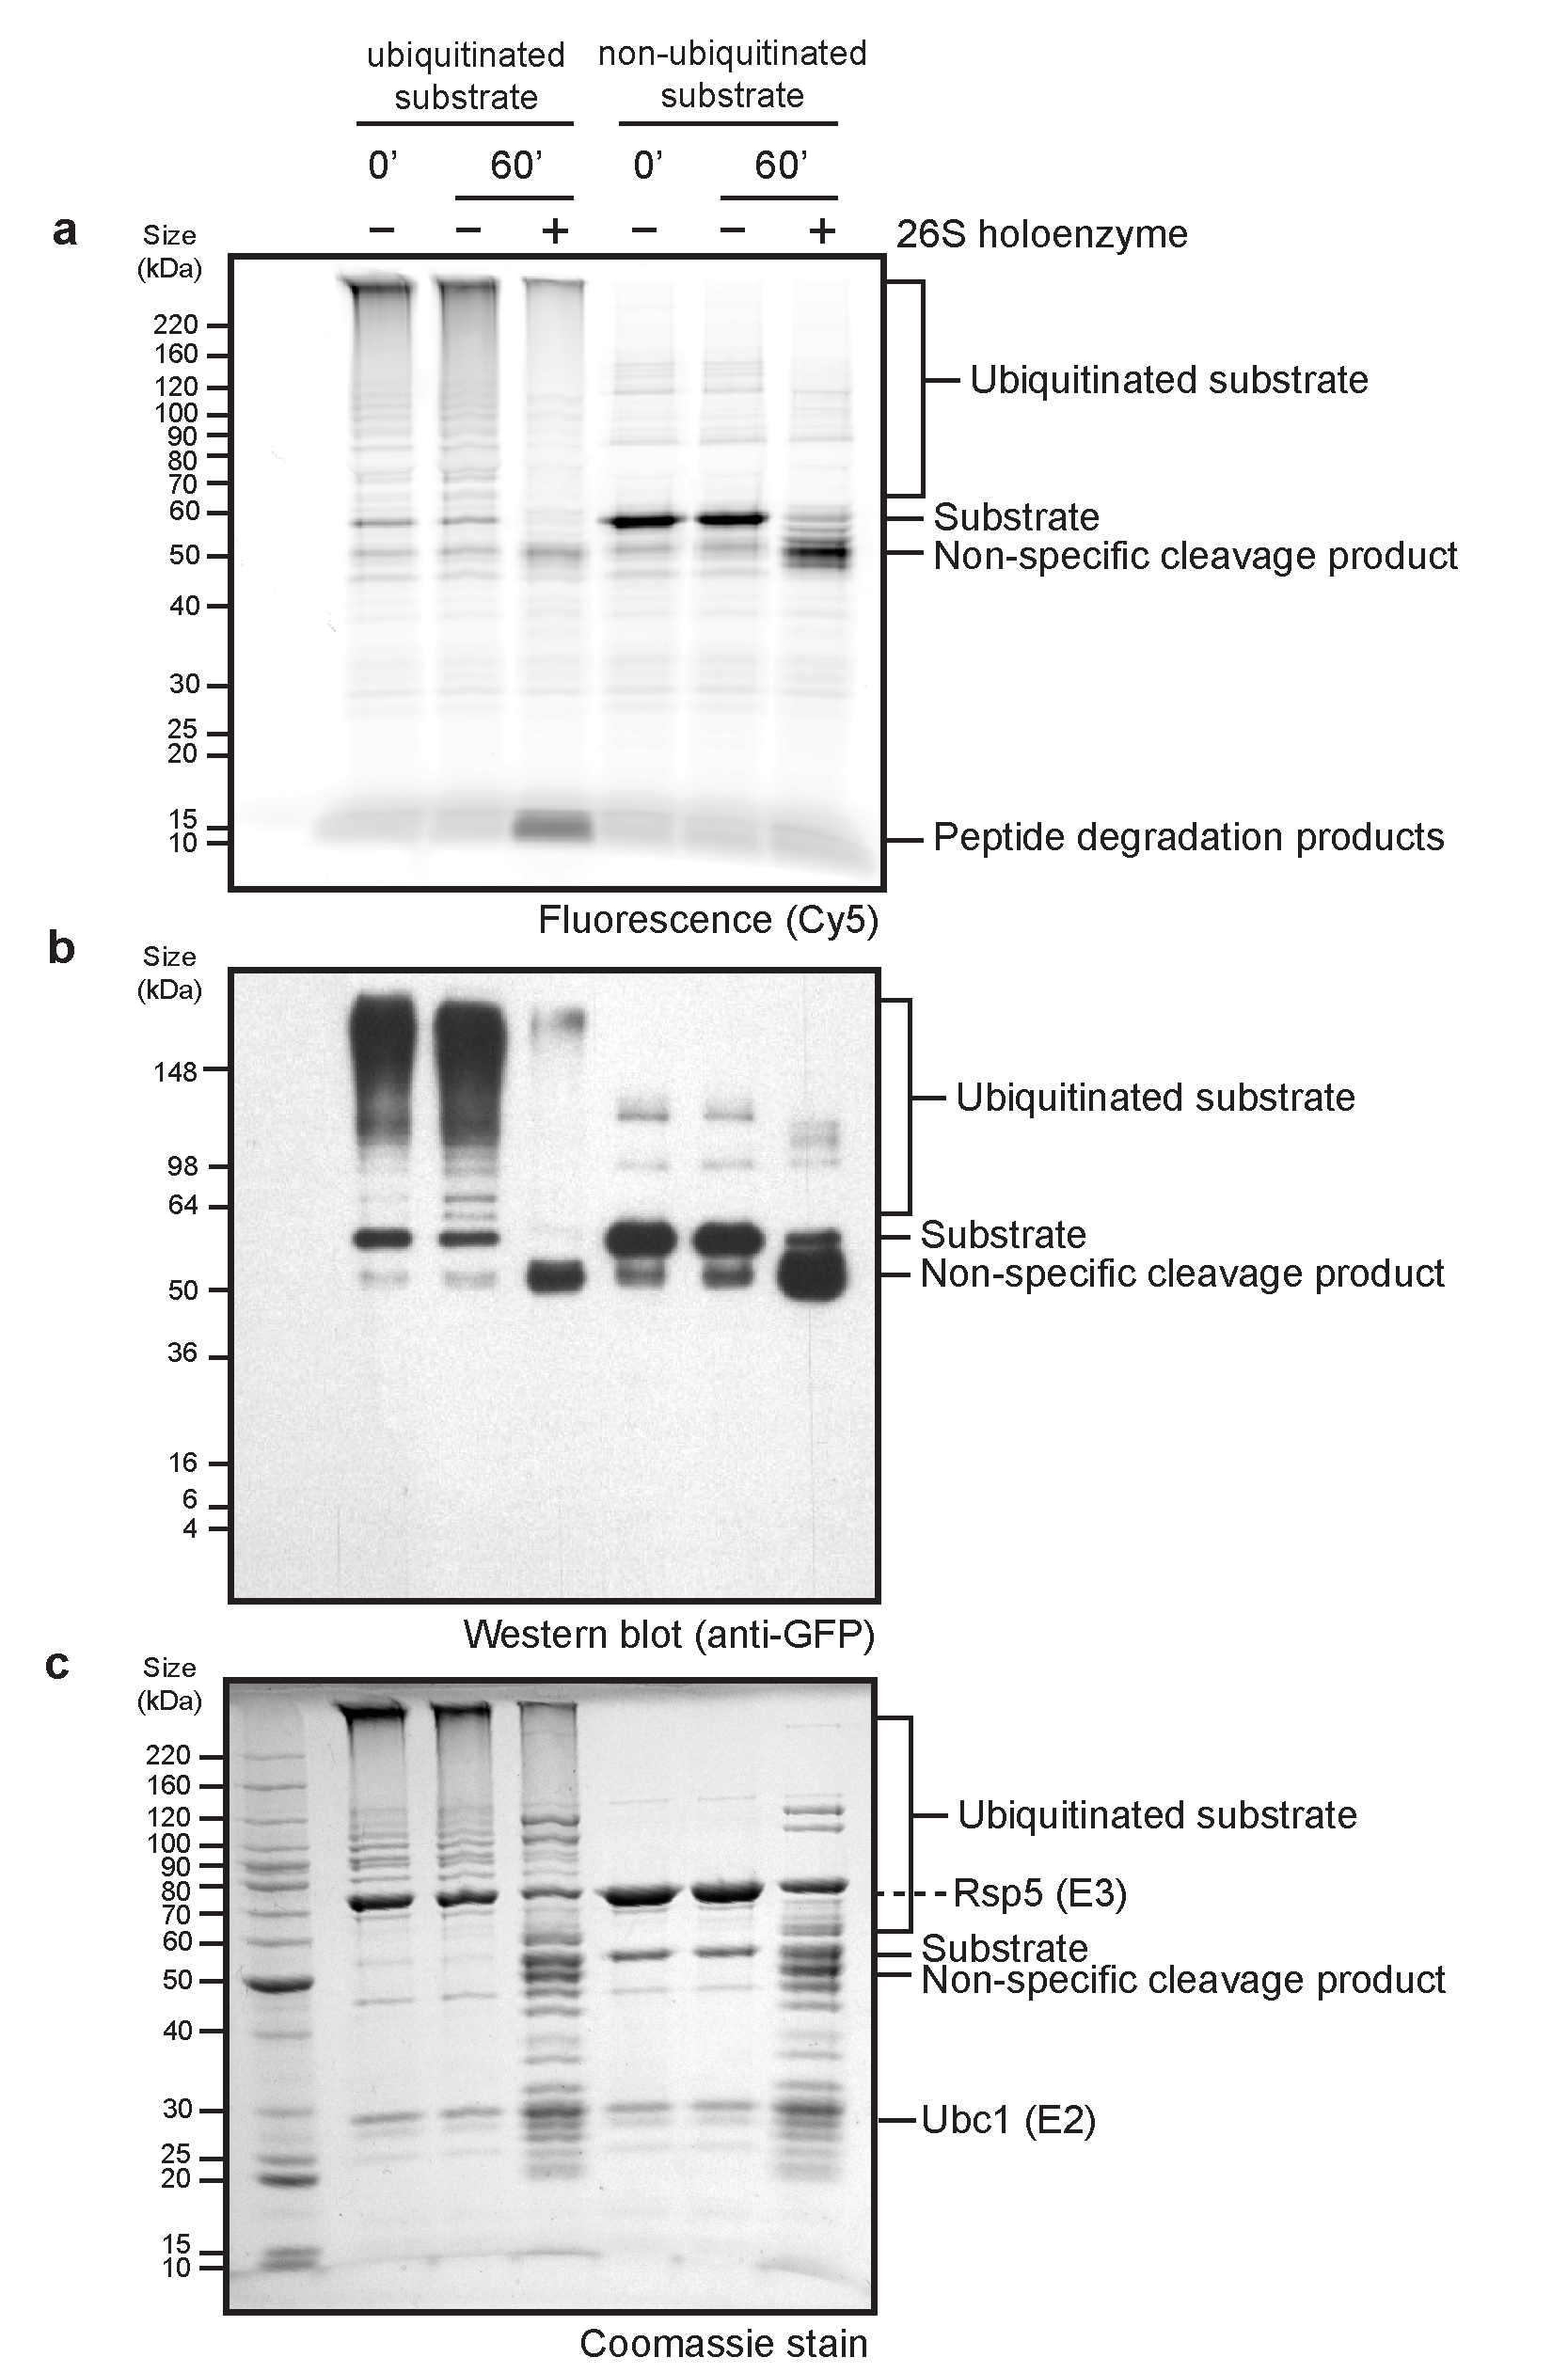
\includegraphics[scale=.36]{gfpdeg}% 
}
\caption[Proteasomal degradation of GFP-fusion substrate]{Proteasomal degradation of GFP-fusion substrate.\par
To demonstrate degradation of the GFP\--titin$^{V15P}$\--cyclin\--PY fusion substrate in a gel-based assay, ubiquitinated or non-ubiquinated substrates were incubated with or without 26S proteasome purified from yeast in the presence of ATP at 30�C for one hour. Samples were then run on a SDS\--PAGE gel followed by (a) fluorescence scanning to detect the Cy5\--label, (b) western blotting using an anti\--GFP antibody, or (c) Coomassie staining for total protein. The fluorescence scan clearly shows the accumulation of small peptide degradation products only for the ubiquitinated substrate in the presence of holoenzyme. Some level of ubiquitin\--independent partial cleavage of an unstructured region of the GFP model substrate was detectable in all three assays. Additional ubiquitination of the substrate was visible in the absence of holoenzyme, which was not unexpected as the enzymes used for \textit{in vitro} ubiquitination of the substrate were still present.}
\label{fig:gfpdeg}
\end{figure}

%-----------------------------

\newpage
\vfill

\begin{figure}[H]
\centering
\setlength{\fboxrule}{0pt}
\fbox{%
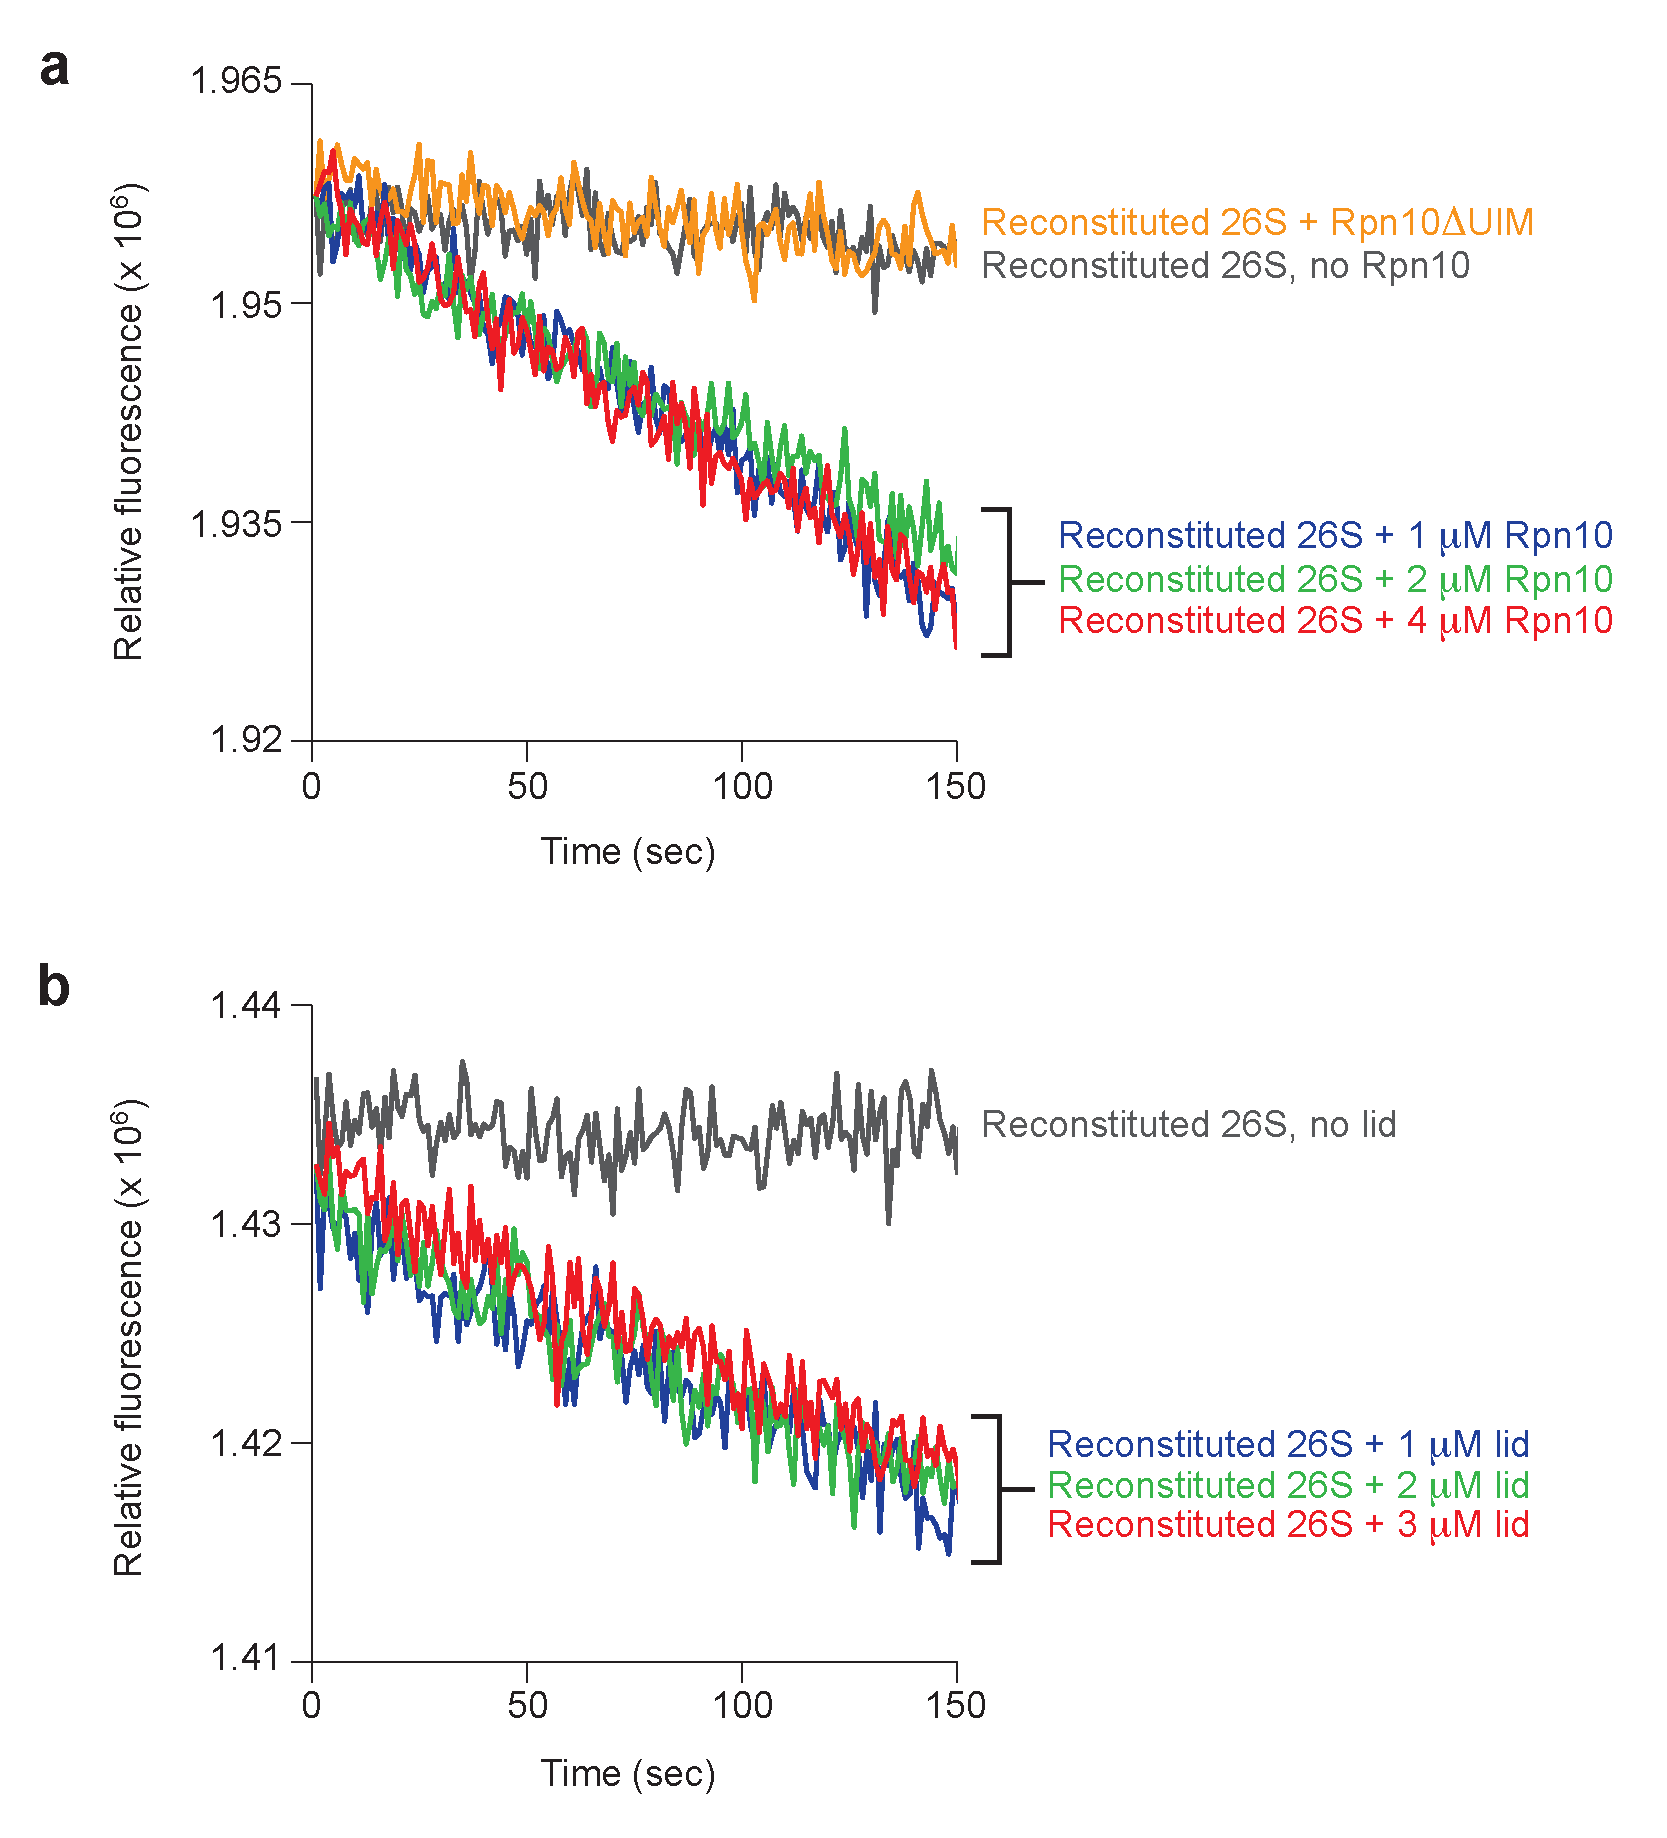
\includegraphics[scale=.45]{degcontrols}% 
}
\caption[Excess lid or Rpn10 do not affect proteasomal degradation rates]{Excess lid or Rpn10 do not affect proteasomal degradation rates.\par
Proteasomal degradation was monitored by the decrease in fluorescence of a polyubiquitinated GFP\--fusion substrate (excitation 467 nm, emission 511 nm) upon incubation with reconstituted 26S proteasome. Degradation reactions contained limiting amounts of core particle (yeast) and \\saturating concentrations of base (\textit{E. coli}\--expressed), lid (yeast), and 1 $\mu$M Rpn10 (\textit{E. coli}\--expressed). To establish that excess amounts of free lid and Rpn10 did not interact with our ubiquitinated substrate and adversely affect the measured degradation rates, we added increasing amounts of \textbf{(a)} Rpn10 or \textbf{(b)} lid and observed that the degradation rate remained constant.}
\label{fig:degcontrols}
\end{figure}


%%-------------------------
\newpage
\vfill

\section{Discussion}
alsdjflaksdjflkjdafs

%%-------------------------


\section{Materials and Methods}

\subsection{Cloning, expression and purification of recombinant base}
Thirteen subunits were cloned into three Novagen vectors including pCOLA\--1 (FLAG\--Rpt1, Rpt2, His$_6$\--Rpt3, Rpt4, Rpt5, Rpt6), pETDuet\--1 (Rpn1, Rpn2, Rpn13), and pACYCDuet\--1 (Nas2, Nas6, Hsm3, Rpn14). Each subunit was preceded by a T7 promoter and all plasmids contained one T7 terminator at the end of the multiple cloning sites. Genes for rare tRNAs were also included in the pACYCDuet\--1 plasmid to account for differences in codon usage between yeast and \textit{E. coli}. Base expression strains were generated by co\--transforming the pETDuet\--1, pCOLA\--1 and pACYCDuet\--1 plasmids into \textit{E. coli} BL21\--star (DE3) cells. The base subcomplex was produced by growing the expression strain to OD$_{600}$=0.6\--0.8 and inducing with 1 mM isopropyl\--b\--D\--thiogalactopyranoside overnight at 18�C. Cells were harvested by centrifugation at 5000 rpm for 15 minutes, resuspended in nickel buffer (25 mM HEPES pH 7.6, 100 mM NaCl, 100 mM KCl, 10\% glycerol, 10 mM MgCl$_2$, 0.5 mM EDTA, 20 mM imidazole) supplemented with 2 mg ml$^{-1}$ lysozyme, protease inhibitors and benzonase. Cells were lysed by freeze\--thaw and sonication on ice for 1 minute 30 seconds in 15 second bursts. Lysate was clarified by centrifugation at 15,000 rpm at 4�C for 30 minutes. A two\--step affinity purification of the base subcomplex was performed using Ni\--NTA agarose (Qiagen) to select for His$_6$\--Rpt3 and anti\--FLAG M2 resin (Sigma\--Aldrich) selecting for FLAG\--Rpt1. 0.5 mM ATP was present in all purification buffers. The Ni\--NTA and anti\--FLAG M2 columns were eluted with nickel buffer containing 250 mM imidazole or 0.15 mg ml$^{-1}$ 3xFLAG peptide, respectively. The Flag column eluate was concentrated using a 30,000 MWCO concentrator (Amicon) and run on a Superose 6 gel filtration column (GE Healthcare) equilibrated with gel filtration buffer (60 mM HEPES pH 7.6, 50 mM NaCl, 50 mM KCl, 10\% glycerol, 5 mM MgCl$_2$, 0.5 mM EDTA, 1 mM DTT, 0.5 mM ATP).  See Appendix~\ref{AppendixB} for detailed protocol.

\subsection{Purification of endogenous yeast complexes}
Yeast holoenzyme, core particle, base and lid subcomplexes were purified from \textit{S. cerevisiae} essentially as previously described~\citep{Leggett2005}. Frozen yeast cells were lysed using a Spex SamplePrep 6870 Freezer/Mill. Holoenzyme was purified from a yeast strain containing FLAG\--Rpn11. Lysed cells were resuspended in lysis buffer containing 60 mM HEPES pH 7.6, 100 mM NaCl, 100 mM KCl, 10\% glycerol, 5 mM MgCl$_2$, 0.5 mM EDTA, 0.2\% NP\--40 and ATP regeneration mix (5 mM ATP, 0.03 mg ml$^{-1}$ creatine kinase, 16 mM creatine phosphate). Holoenzyme was bound to anti\--FLAG M2 resin and washed with wash buffer (60 mM HEPES pH 7.6, 100 mM NaCl, 100 mM KCl, 10\% glycerol, 5 mM MgCl$_2$, 0.5 mM EDTA, 0.1\% NP-40, 0.5 mM ATP). Holoenzyme was eluted with 0.15 mg ml$^{-1}$ 3xFLAG peptide and further purified by gel filtration using a Superose 6 column with gel filtration buffer (see above). Lid and base subcomplexes were isolated from FLAG\--Rpn11 or FLAG\--Rpn2 yeast strains, respectively, and purified by exposure to a 1 M NaCl wash while bound to anti\--FLAG M2 resin. Base purification buffers included 0.5 mM ATP. Core particle was purified from a 3xFLAG\--Pre1 yeast strain using a 500 mM salt wash. All subcomplexes underwent size exclusion chromatography using a Superose 6 column as described above.

\subsection{Yeast strains}
Yeast lid and holoenzyme were purified from strain YYS40 (genotype MATa ade2\--1 his3\--11,15 leu2\--3,112 trp1\--1 ura3\--1 can1 Rpn11::Rpn11\--3XFLAG(HIS3), source Y. Saeki). Core particle was prepared either from strain RJD1144 (genotype MATa his3\--200 leu2\--3,112 lys2\--801 trp\--63 ura3\--52 PRE1\--FLAG\--6xHIS::Ylpac211(URA3) source R. Deschaies) or strain yAM14 (genotype MATa ade2\--1 his3\--11,15 leu2\--3,112 trip1\--1 ura3\--1 can1\--100 bar1 PRE1::PRE1\--3XFLAG(KanMX), this work).

\subsection{Native gel electrophoresis}
Analysis of proteasome holoenzyme and subcomplexes by native gel was performed as described previously~\citep{Leggett2005}. Assembly reactions were incubated for 15 minutes at 23�C with 5 mM ATP, followed by electrophoresis on a 3.5\% native polyacrylamide gel. Electrophoresis was conducted at 4�C with stirring and running buffer containing 0.5 mM ATP. The gel was overlaid with developer solution (running buffer with 100 nM Suc\--LLVY\--AMC peptide (Boston Biochem) and 0.02\% SDS) and incubated at 30�C for 10 minutes prior to imaging. Fluorescence imaging was performed using a Typhoon scanner (GE Healthcare) and followed by Coomassie staining.

\subsection{ATPase and peptidase stimulation assays}
ATPase activity was quantified using an NADH\--coupled ATPase assay. 500 nM base was incubated with 1x ATPase mix (3 U ml$^{-1}$ pyruvate kinase, 3 U ml$^{-1}$ lactate dehydrogenase, 1 mM NADH, 7.5 mM phosphoenol pyruvate) at 30�C. Absorbance at 340 nm was monitored for 900 seconds at 10 second intervals using a UV\--Vis Spectrophotometer (Agilent). Peptidase stimulation was monitored by following the increase in fluorescence resulting from cleavage of a fluorogenic peptide substrate~\citep{Glickman1998}, Suc\--LLVY\--AMC (Boston Biochem), using a QuantaMaster spectrofluorimeter (PTI). 50 nM core particle was incubated with saturating base subcomplex in the presence of an ATP regeneration system (5 mM ATP, 16 mM creatine phosphate, 6 mg ml$^{-1}$ creatine phosphokinase) and 50 $\mu$M Suc-LLVY-AMC.

\subsection{Gel-based substrate degradation assay}
The model substrate, a green fluorescent protein (GFP)\--titin$^{V15P}$\--cyclin\--PY, was labeled at the N-terminus with Cy5 dye and subsequently modified with a polyubiquitin chain in vitro using Uba1, Ubc1, Rsp5 and wild\--type ubiquitin. The non\--ubiquitinated substrate was prepared similarly except ubiquitin was omitted from the reaction. Degradation was assessed by incubating substrates with 26S holoenzyme purified from yeast in the presence of an ATP regeneration system at 30�C for one hour. Substrate degradation was then assessed by running samples on a SDS\--PAGE gel followed by fluorescence scanning to detect the Cy5\--labeled substrate (670 nm band\--pass 30 filter), western blotting using an anti\--GFP antibody, or Coomassie staining for total protein.

\subsection{Fluorescent substrate degradation assay}
Proteasome holoenzyme was reconstituted from core particle, lid, base and Rpn10. A GFP\--titin$^{V15P}$\--cyclin\--PY fusion protein was modified \textit{in vitro} with a polyubiquitin chain using Uba1, Ubc1, Rsp5 and wild-type ubiquitin. Degradation reactions were performed at 30�C in gel filtration buffer (60 mM HEPES pH 7.6, 50 mM NaCl, 50 mM KCl, 10\% glycerol, 5 mM MgCl$_2$, 0.5 mM EDTA, 1 mM DTT, 0.5 mM ATP) supplemented with an ATP regeneration system. Degradation activities were monitored by the loss of GFP fluorescence (excitation 467 nm; emission 511 nm) using a QuantaMaster spectrofluorimeter (PTI). Multiple turnover degradation experiments were performed with 50 nM reconstituted holoenzyme under V$_{max}$ conditions (saturating base, lid and Rpn10) with 2 $\mu$M substrate. Excess base, lid, and Rpn10 did not affect the observed degradation rate (see Figure \ref{fig:degcontrols} for lid and Rpn10).

%%-------------------------





% Chapter 3

\chapter{Functional asymmetry of the proteasomal AAA+ unfoldase} % Write in your own chapter title
\label{Chapter3}
\lhead{Chapter 3. \emph{Functional asymmetry of the proteasomal AAA+ unfoldase}} % Write in your own chapter title to set the page header


\section{Introduction}
The ubiquitin\--proteasome system (UPS) is the major pathway for selective protein degradation in all eukaryotic cells, where it mediates protein quality control and the destruction of critical regulatory proteins~\citep{Hochstrasser1996,Finley2009}.  Protein substrates are covalently modified with a poly\--ubiquitin chain and targeted to the 26S proteasome for ATP\--dependent proteolysis. Despite this crucial role of the UPS for protein degradation, the mechanistic principles of the proteasome still remain largely elusive.\par

The eukaryotic 26S proteasome is a 2.5 MDa molecular machine formed from at least 33 different subunits. It consists of a barrel\--shaped 20S core particle that is capped on one or both ends by the 19S regulatory particle. The core particle contains an internal chamber with sequestered proteolytic active sites and gated axial pores to restrict substrate entry~\citep{Groll2000}. Access to this chamber is controlled by the regulatory particle, which is also responsible for recognition, deubiquitination, engagement, unfolding, and translocation of substrate~\citep{Glickman1998,Thrower2000,Liu2006,Smith2007}. The regulatory particle includes 19 different subunits and can be divided into the base and lid subcomplexes. The base contains a ring of six distinct AAA$+$ ATPases in the order Rpt1\--2\--6\--3\--4\--5~\citep{Tomko2010,Tomko2011}, which constitute the ATP\--dependent motor of the proteasome and dock atop the core particle. Additional integral components of the base are the ubiquitin receptor Rpn13 as well as two large scaffolding subunits, Rpn1 and Rpn2~\citep{Hamazaki2006,Beck2012,Lander2012}. The nine\--subunit lid, which includes the deubiquinating enzyme Rpn11~\citep{Verma2002,Yao2002}, binds asymmetrically to the side of the base\--core complex and positions the second ubiquitin receptor, Rpn10, close to the lid\--base interface above the entrance of the processing pore~\citep{Beck2012,Lander2012,Sakata2012}\par

Once a substrate is tethered to a proteasomal ubiquitin receptor, a complex set of enzymatic activities defines the pathway to degradation. The substrate must be deubiquitinated by Rpn11, while the ATPase ring of the base engages an unstructured degradation-initiation region of the protein, mechanically disrupts globular structures, and translocates the unfolded polypeptide into the peptidase chamber. ATP hydrolysis by the Rpt subunits of the base is crucial for substrate degradation, yet it remains unclear how these six distinct subunits work together to drive ATP\--dependent unfolding and translocation. \par

Previous studies of the related homohexameric unfoldase ClpX suggest that ATP hydrolysis occurs in one subunit at a time with a certain degree of coordination, such that subunits may contribute additively and equally to substrate processing~\citep{Martin2005}. However, the homomeric nature of ClpX hinders assessment of whether all six subunits indeed sequentially progress through the different stages of the ATP\--hydrolysis cycle. The unique heterohexameric architecture of the proteasomal ATPase ring has thus prompted the fundamental question whether the six Rpts are functionally equivalent or play distinct roles in ATP hydrolysis and substrate processing. While Rpt1\--6 share highly homologous AAA$+$ ATPase domains, they differ substantially in their N-terminal coiled-coil domains, which interact with the laterally bound lid, and in their C\--terminal unstructured tails, which mediate interaction with the core particle and trigger gate opening to the proteolytic chamber~\citep{Smith2007,Gillette2008,Rabl2008,Kim2011}.  Furthermore, recent EM structures of the apo and substrate\--bound 26S proteasome revealed distinct vertical asymmetries within the base ATPase ring~\citep{Beck2012,Lander2012,Matyskiela2013,Sledz2013}. In the absence of substrate, the large AAA$+$ subdomains of Rpt1\--6 adopt a pronounced spiral-staircase configuration, with Rpt3 at the top and Rpt2 at the bottom position.  Strikingly, upon substrate engagement, the base switches to a more planar ring conformation that is characterized by a spiral staircase with Rpt1 at the top and Rpt4 at the bottom~\citep{Matyskiela2013}. However, the functional significance of these staircase configurations, potentially manifested as differential subunit contributions to substrate degradation or subcomplex interactions within the holoenzyme, has yet to be determined. \par

Endogenous 26S proteasome has been used to investigate the role of individual Rpts, revealing functional differences in their contributions to base assembly, 26S holoenzyme formation, ATP hydrolysis, peptidase gate opening, and substrate degradation~\citep{Rubin1998,Kohler2001,Smith2007,Park2009,Thompson2009,Kumar2010,Erales2012,Kim2012,Lee2012}. Despite these results, limitations in working with endogenous proteasome, in part due to \textit{in\--vivo} assembly problems or lethal degradation defects, have largely prevented extensive systematic studies and a quantitative mechanistic understanding of the individual processes involved in substrate degradation.\par 

Here, we investigated the mechanisms underlying ATP\--dependent substrate processing by the heterohexameric unfoldase of the 26S proteasome. To define the differential contributions of individual Rpts to ATP hydrolysis, substrate degradation, peptidase binding, and gate opening, we developed systems for the heterologous expression of the base subcomplex and the \textit{in\--vitro} reconstitution of partially recombinant proteasomes, and performed systematic mutational analyses of key catalytic and structural motifs. \par

%%-------------------------

\section{Results}

\subsection{Distinct roles of individual ATPase subunits in substrate processing}
%fig MTO and STO deg
%table

To examine the roles of Rpt1\--6 in nucleotide\--dependent substrate processing, we individually abolished their ATP hydrolysis by systematically introducing a catalytic mutation in the recombinant base. In the homohexameric bacterial unfoldase ClpX, mutation of the conserved Walker\--B  glutamate prevents hydrolysis and induces a permanently ATP\--bound state in the mutated subunit~\citep{Hersch2005}, but other AAA+ unfoldases require distinct Walker\--B mutations to eliminate ATP\--hydrolysis activity~\citep{Gomez2002,Weibezahn2004}. We therefore tested the effects of various substitutions of the conserved Walker\--B aspartate and glutamate residues by simultaneously placing them in all six Rpts (see Section~\ref{methods:mutations}). Ultimately, mutation of glutamate to glutamine (EQ) allowed proper assembly of base that exhibited wild\--type levels of peptidase\--binding and gate\--opening activities despite being inactive in ATP hydrolysis (Table~\ref{table:alldata}), indicating that this mutation in fact traps Rpt subunits in a permanently ATP\--bound state. We next introduced a single EQ mutation per hexamer to fix individual Rpts in the ATP\--bound state and test their contributions to ATP hydrolysis as well as core-gate opening. Depending on which subunit was mutated, we observed considerable differences in activities (Table~\ref{table:alldata}), indicating that the Rpt subunits are functionally non-equivalent.\par

ATP hydrolysis by the isolated base decreased by more than 60\% upon mutation of Rpt3, whereas inactivating other subunits had either minor effects (Rpt1, Rpt4, Rpt5) or notably increased the hydrolysis rate (Rpt2, Rpt6). Peptidase stimulation by these base mutants also varied: mutated Rpt5, Rpt2, and Rpt6 caused 20\%, 30\%, and 60\% stronger gate opening compared to wild\--type base, mutated Rpt4 did not lead to noticeable changes, while mutations in Rpt3 or Rpt1 decreased gate\--opening activity by 20\% or 30\% despite proper complex formation with the core particle. It is important to consider that the measured ATPase and gate\--opening activities reflect an average of the unmutated five Rpt subunits and are influenced by subunit communication. The increase in ATPase activity resulting from mutation of Rpt2 and Rpt6, for instance, is likely caused by the response of neighboring subunits to a permanently ATP\--bound state. Some of these stimulated ATP\--hydrolysis events may be non\--productive and thus not result in increased substrate\--degradation rates. This is supported by the fact that most base variants containing a mutant Rpt showed no stimulation or even slight repression in ATP\--hydrolysis activity upon the addition of substrate, whereas the ATPase rate of wild\--type base approximately doubled (Figure~\ref{fig:eqatpase}). \par

%%-------------------------
\begin{figure}[h!]
\centering
\subfigure{%
	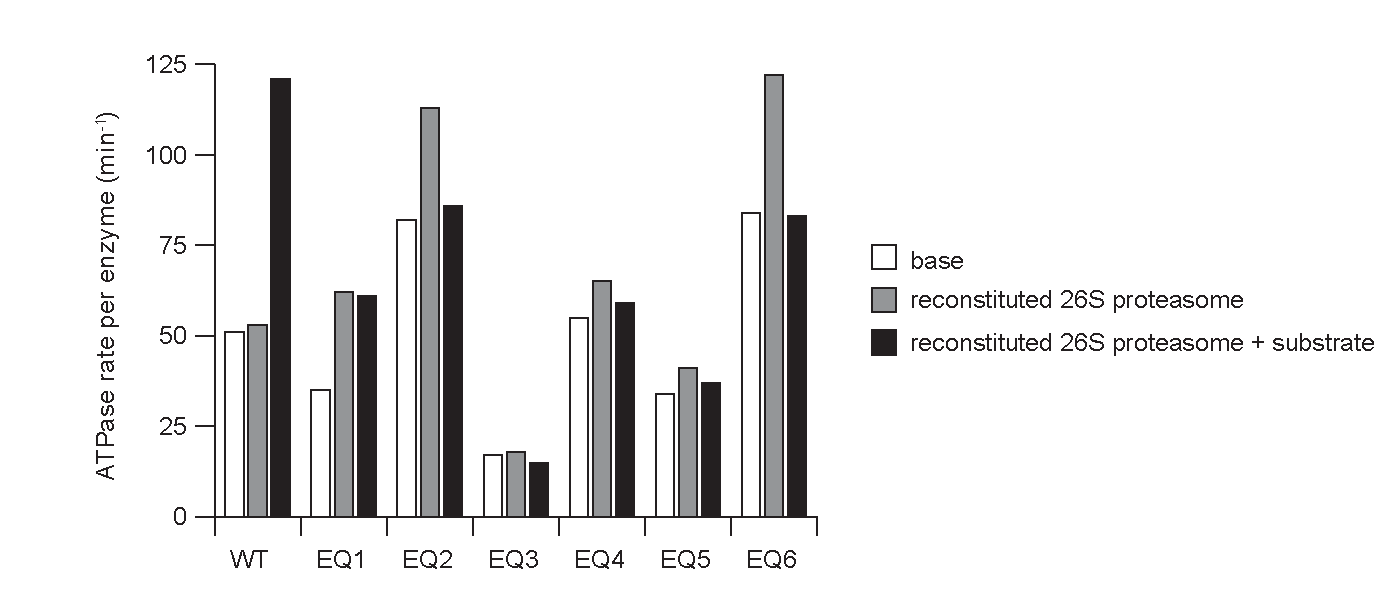
\includegraphics[width=1\linewidth]{workingatpase}
	\label{fig:workingatpase}}
\quad	
\subfigure{%
\vspace{10pt}
\begin{tabular*}{\textwidth}{@{}lcccccccc@{}}\toprule
\phantom{a} & \multicolumn{2}{C{4cm}}{basal ATPase rate (base)} & \phantom{a}& \multicolumn{2}{C{4cm}}{basal ATPase rate (reconstituted 26S)} & 
\phantom{a} & \multicolumn{2}{C{5.65cm}}{working ATPase rate (reconstituted 26S proteasome + ubiquitinated substrate}\\
\cmidrule{2-3} \cmidrule{5-6} \cmidrule{8-9}
\phantom{a} & min$^{\--1}$ & \% WT & & min$^{\--1}$ & \% WT & & min$^{\--1}$ & \% WT\\ \midrule
WT & 51 & 100 & & 53 & 103 & & 121 & 237\\
EQ1 & 35 & 68 & & 62 & 122 & & 61 & 120\\
EQ2 & 82 & 161 & & 113 & 221 & & 86 & 169\\
EQ3 & 17 & 33 & & 18 & 36 & & 15 & 28\\
EQ4 & 55 & 108 & & 65 & 127 & & 59 & 116\\
EQ5 & 34 & 67 & & 41 & 81 & & 37 & 72\\
EQ6 & 83 & 164 & & 122 & 240 & & 83 & 162\\
\bottomrule
\end{tabular*}
	\label{table:workingatpase}}
%
\caption[ATP hydrolysis rates for Walker\--B EQ mutant base subcomplexes are not stimulated by ubiquitinated substratese]{ATP hydrolysis rates for Walker\--B EQ mutant base subcomplexes are not stimulated by ubiquitinated substrate.\par
Stimulation of ATPase activity by the base in the presence of ubiquitinated substrate was determined using a NADH\--coupled ATPase assay. \textbf{(a)} Basal rates of ATP hydrolysis per enzyme (base hexamer) were determined both for base subcomplexes alone (white) and reconstituted 26S proteasomes containing the base variants (gray).  Working ATPase rates were measured by adding ubiquitinated substrate to reactions containing reconstituted 26S proteasomes (black). \textbf{(b)} Table expressing the data from (a) in terms of ATP hydrolyzed per enzyme per minute and as a percentage of the rate observed for wild\--type (WT) base alone. Errors for the ATPase assay were estimated to be $\pm$10\% of the WT mean value.
}
\label{fig:eqatpase}
\end{figure}
%%-------------------------

%%-------------------------
\newpage
\vfill
\begin{figure}[H]
\centering
\subfigure{%
	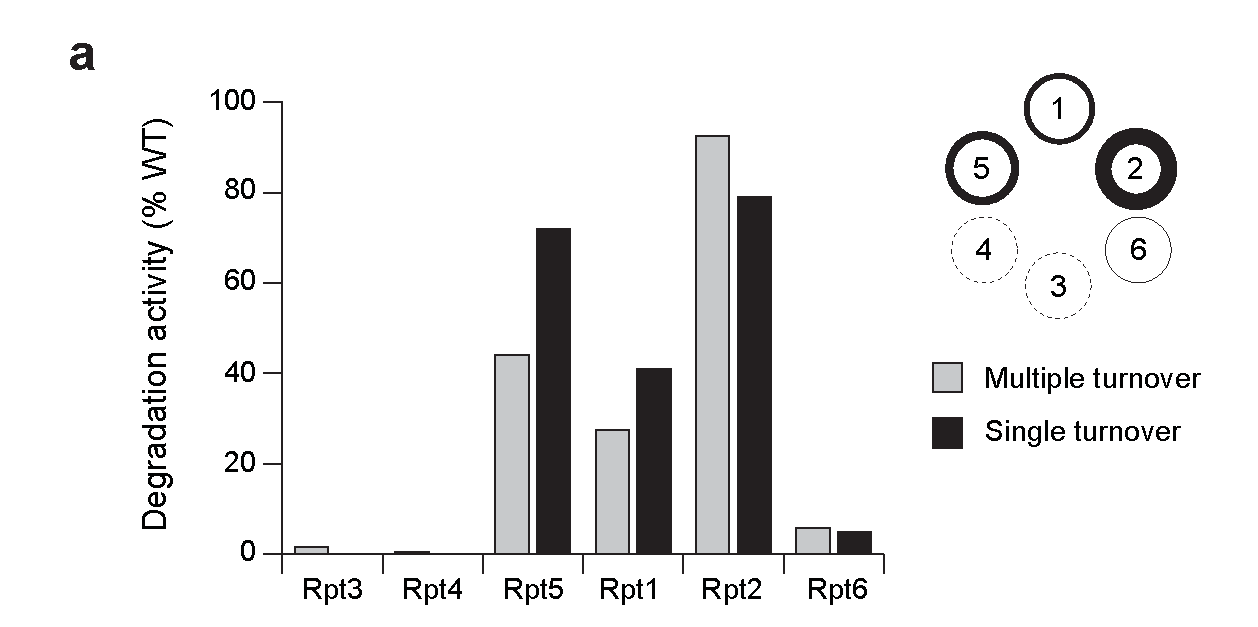
\includegraphics[scale=0.46]{walkerbdeg}
	\label{fig:wbdeg}}
\quad	
\subfigure{%
	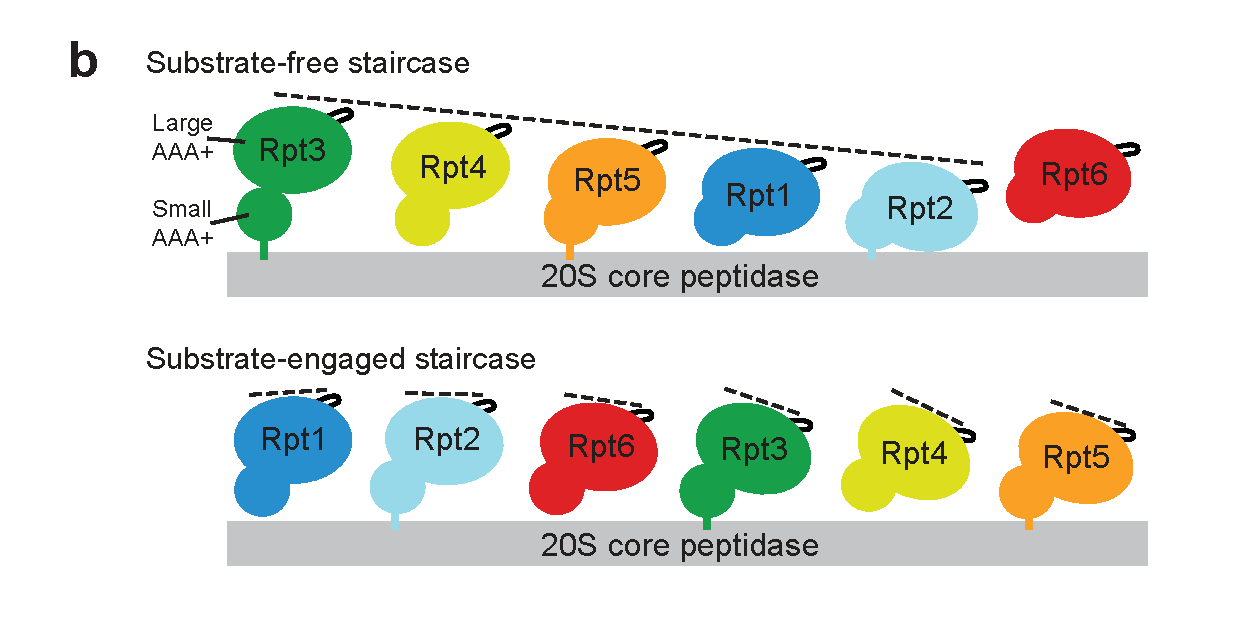
\includegraphics[scale=0.46]{staircase}
	\label{fig:staircase}}
%
\caption[Degradation activities for base variants with a Walker\--B mutation in individual Rpt subunits correlate with the subunit's position in the spiral staircase arrangement of the base]{Degradation activities for base variants with a Walker\--B mutation in individual Rpt subunits correlate with the subunit's position in the spiral staircase arrangement of the base.\par
\textbf{(a)} \textit{In vitro} degradation rates for reconstituted proteasomes containing base variants with single Rpt subunits fixed in a permanent ATP\--bound state by the E$\rightarrow$Q mutation. Degradation under multiple\--turnover (gray) and single\--turnover (black) conditions was monitored by the loss of fluorescence resulting from the degradation of a polyubiquitinated GFP fusion substrate. Degradation activities were measured relative to that of the reconstituted proteasome containing wild\--type (WT) recombinant base. Errors for multiple\--turnover degradation rates were estimated to be $\pm$10\% (s.d.) of the mean WT value on the basis of repeat measurements (n = 3 technical replicates). The circular diagram is an alternative representation of the multiple\--turnover data, with each number referring to the respective Rpt subunit and the line thickness corresponding to the observed degradation activity for a mutation in that subunit. \textbf{(b)} The large AAA+ subdomains of Rpt1\--Rpt6 adopt distinct spiral staircase arrangements in the absence or presence of substrate. Shown are cartoon representations of the pre\--engaged (top) and substrate\--engaged (bottom) staircases based on cryo\--EM reconstructions9, 20, with the individual Rpt subunits splayed out and their pore\--facing sides pointing to the right. In the pre\--engaged spiral, the small AAA+ subdomains of Rpt1\--Rpt6 are arranged in a relatively planar fashion, whereas the large AAA+ subdomains are differentially lifted out of the ring plane, resulting in a pronounced spiral staircase with Rpt3 in the highest position and Rpt2 in the lowest position. In the substrate\--engaged spiral, the small and large AAA+ subdomains are mostly level, and the staircase orientation of the pore loops originates primarily from differential rotations of subdomains in the plane of the ring.
}
\label{fig:wbdegstaircase}
\end{figure}
%%-------------------------


%%-------------------------
\begin{figure}[b!]
\centering
\subfigure{%
	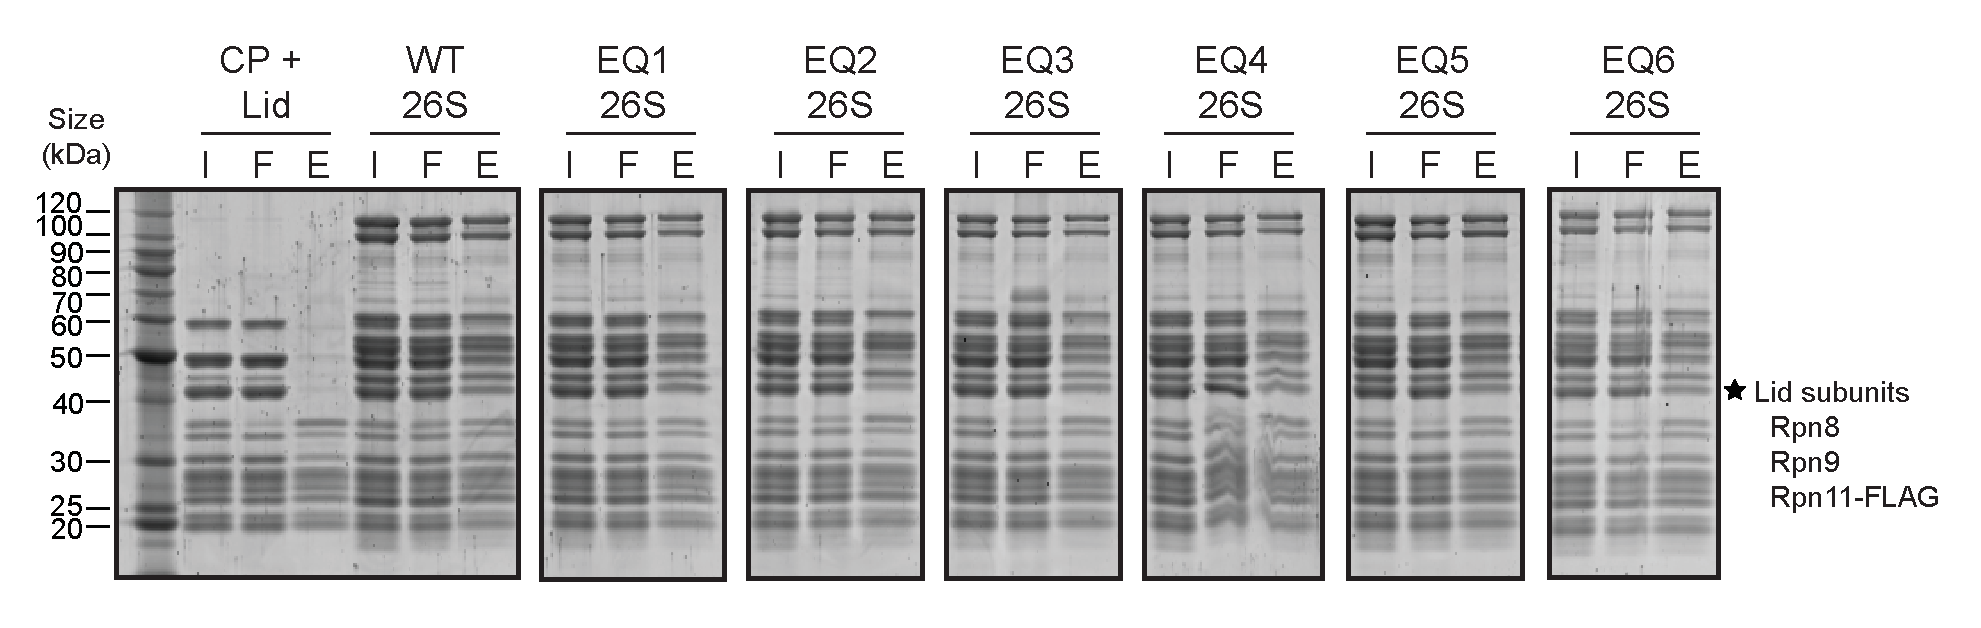
\includegraphics[scale=0.5]{wbpulldown}
	\label{fig:wbpulldown}}
\quad	
\subfigure{%
	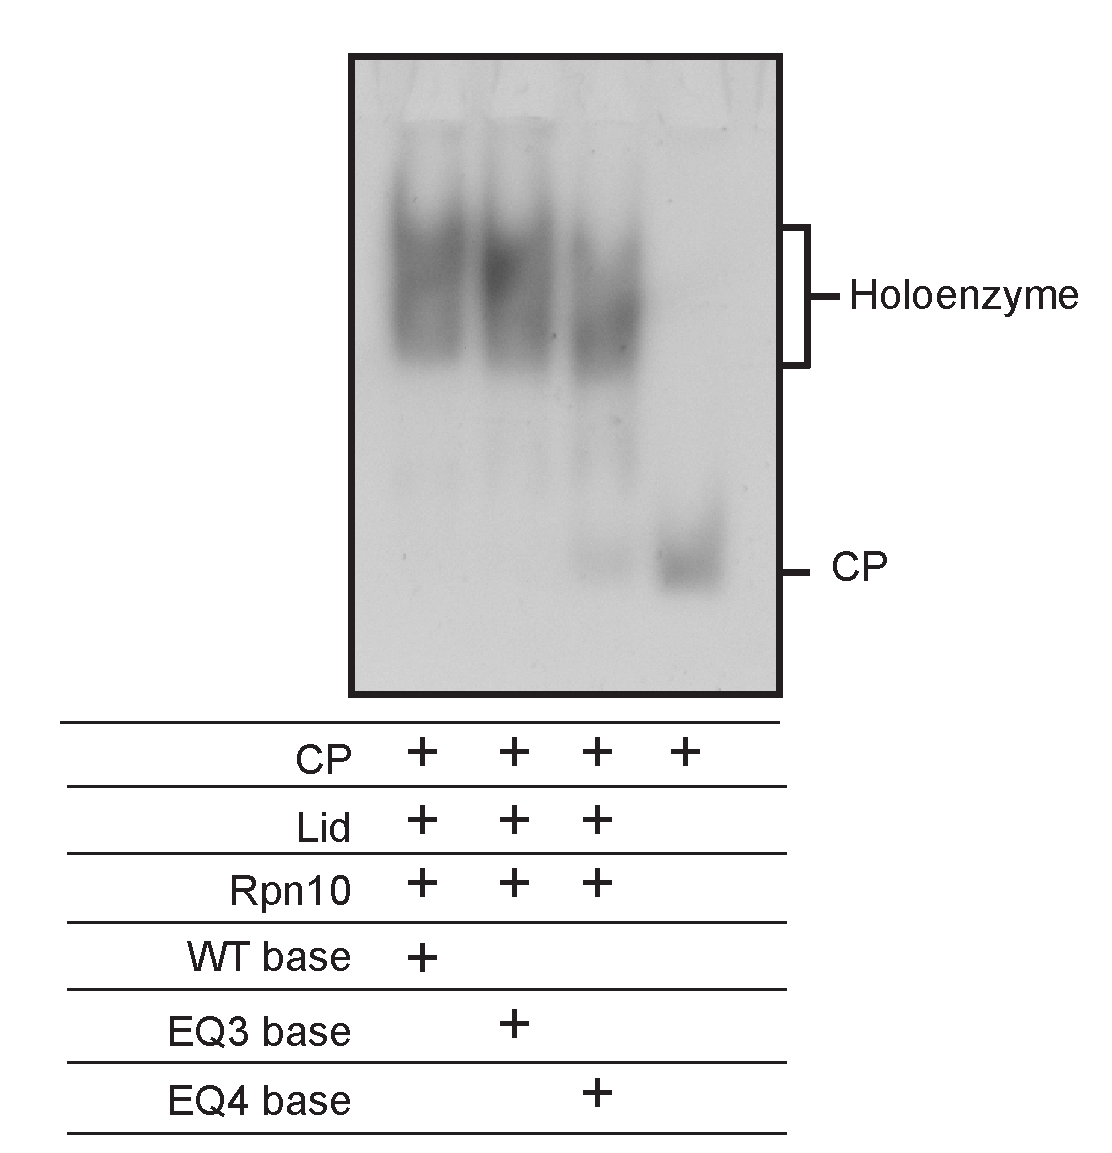
\includegraphics[scale=0.4]{wbnative}
	\label{fig:wbnative}}
%
\caption[title]{title.\par
\textbf{(a)} first caption. \textbf{(b)} second caption.
}
\label{fig:wbctls}
\end{figure}
%%-------------------------

To explore the distinct roles of individual Rpt subunits in substrate processing, we reconstituted proteasomes with base variants containing single\--subunit EQ mutations and compared their rates of ubiquitin\--mediated substrate degradation under multiple\--turnover conditions (Figure \ref{fig:wbdeg}). An EQ mutation in either Rpt3 or Rpt4 completely eliminated substrate degradation, and a mutated Rpt6 resulted in a 90\% decrease in degradation rate. Mutations in Rpt1 and Rpt5 lowered the degradation rate by 73\% and 56\%, respectively, whereas the Rpt2 mutant showed no defect. Importantly, the observed degradation defects were not simply the result of compromised proteasome assembly, as all mutants stimulated peptidase\--gate opening (Table~\ref{table:alldata}) and bound lid and core particle (Supplementary Fig. 5a,b). Considering the order of ATPase subunits within the base (Rpt1\--2\--6\--3\--4\--5), it is strikingly evident that mutants with severe degradation defects (Rpt6, Rpt3, and Rpt4) map to one half of the ring. \par

%%-------------------------
\begin{figure}[b!]
\centering
\setlength{\fboxrule}{0pt}
\fbox{%
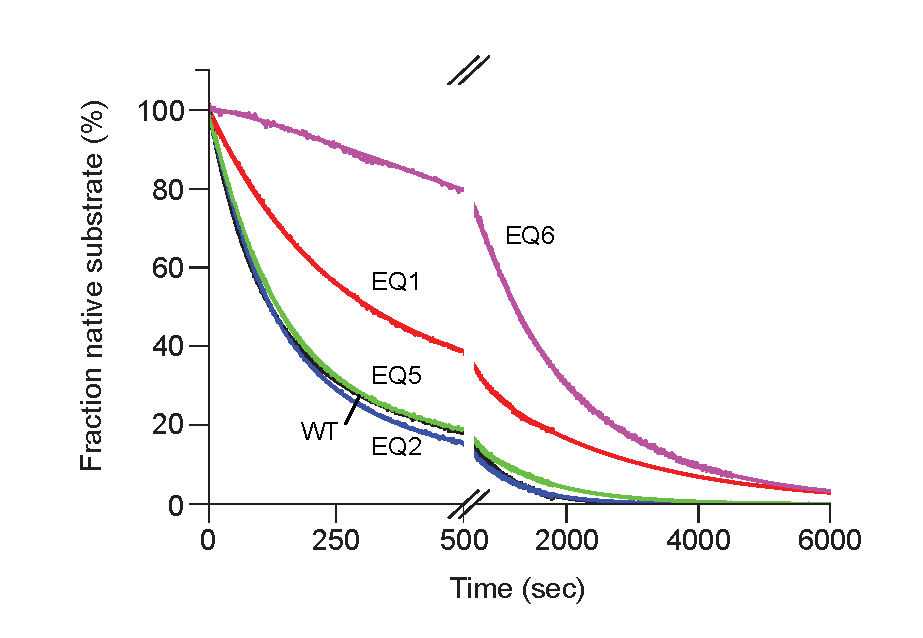
\includegraphics[scale=.75]{wbsto}% 
}
\caption[title]{title.\par
Single\--turnover degradation traces and curve fits for EQ base mutants. Degradation under single\--turnover conditions was monitored by the decrease in fluorescence of 100 nM polyubiquitinated GFP\--fusion substrate (excitation 467 nm, emission 511 nm) upon incubation with 2 $\mu$M 26S proteasome reconstituted with either WT base or EQ base variants. Proteasomes reconstituted with EQ3 or EQ4 base variants did not exhibit any measurable degradation even under single turnover conditions. Curves were best fit with a double exponential decay, likely reflecting degradation of two subpopulations of the substrate. These classes of substrate probably differ in the number or location of conjugated polyubiquitin chains but their affinity for the proteasome is expected to be similar. 
}
\label{fig:wbsto}
\end{figure}
%%-------------------------



Next we investigated the mechanistic role of individual Rpts at different stages of substrate processing by performing single\--turnover degradation experiments (Figure \ref{fig:wbdeg}, Figure \ref{fig:wbsto}). In contrast to steady\--state analyses, these measurements discriminate between potential defects in substrate engagement versus translocation and unfolding. The resulting data for GFP\--substrate turnover were best fit by a double\--exponential decay. Since GFP loses fluorescence in a single unfolding step, this double\--exponential behavior was likely due to two types of substrates that probably varied in their ubiquitin tagging and were degraded at different rates. As expected, the two rates averaged to roughly match the multiple\--turnover rate, and the base mutants exhibited the same ranking of activities as in multiple\--turnover degradation (Figure \ref{fig:wbdeg}, Table~\ref{table:alldata}). Even under these single-turnover conditions, Rpt3 or Rpt4 mutants did not show any measurable degradation, whereas the Rpt6 mutant degraded substrate at 5\% of the wild\--type rate. This Rpt6 mutant exhibited a short lag preceding the exponential fluorescence decay (Figure \ref{fig:wbsto}), which may indicate delayed substrate translocation and unfolding due to defects in engagement. The 95\% decrease in degradation rate may thus originate from slower engagement instead of or in addition to compromised unfolding and translocation. The complete lack of substrate degradation for ATPase\--deficient Rpt3 or Rpt4 may similarly be a consequence of severe engagement defects.



\subsection{Spiral staircase configuration of ATPase large AAA+ domains}
%fig staircase

EM reconstructions of the ATP\--bound 26S proteasome in the absence of substrate revealed that the large AAA+ subdomains of the Rpts adopt a pronounced spiral\--staircase configuration around the ring~\citep{Beck2012,Lander2012}. Rpt3 occupies the highest and Rpt2 the lowest position relative to the core particle, with Rpt6 bridging the vertical gap between the two subunits (Figure \ref{fig:staircase}). The degradation defects of EQ mutants and the inferred contributions of individual Rpts to substrate degradation largely correlate with the vertical positions of subunits in this pre\--engaged staircase. Conformational changes in subunits at the top of the apo spiral (Rpt3, Rpt4 and Rpt6) thus appear to be critical to engage a substrate and initiate translocation, whereas subunits in lower positions are less important. \par

Our recent EM reconstruction of the translocating proteasome~\citep{Matyskiela2013} demonstrated that substrate engagement induces substantial conformational changes in the regulatory particle, leading to a more planar ATPase\--ring with a rearranged staircase of pore loops, in which Rpt1 is at the top and Rpt4 at the bottom position (Figure \ref{fig:staircase}). Based on the static appearance of the spiral, in combination with single\--molecule data for the related protease ClpXP, we previously proposed that the substrate\--engaged staircase represents a default dwell state that is adopted by the base before or after coordinated ATP\--hydrolysis events progress around the ATPase ring~\citep{Matyskiela2013}. Interestingly, in the present study we observed an approximately 70\% reduction in degradation activity when ATP hydrolysis was eliminated in Rpt1, located at the top of the substrate\--engaged staircase. Rpt1 may therefore play a special role in processive substrate translocation, possibly by triggering the coordinated ATP hydrolysis of subunits.

\subsection{Contribution of individual pore loops to substrate processing}
%fig pore loops
%table
Previous work on various AAA+ unfoldases proposed that a conserved aromatic\--hydrophobic (Ar\--$\phi$) loop protrudes from every ATPase subunit into the central channel and undergoes nucleotide-dependent power strokes to drive substrate translocation~\citep{Wang2001,Yamada2003,Hinnerwisch2005,Park2005,Martin2008a, Martin2008b,Aubin2011,Maillard2011,Erales2012}. To study these loop functions in the proteasome, we constructed base variants with tyrosine\--to\--alanine mutations in the Ar\--$\phi$ loop of individual Rpts (Table~\ref{table:alldata}, Figure \ref{fig:pore1loops}). Loop mutations in Rpt3, Rpt4, or Rpt6 decreased the rate of ATP hydrolysis by 15\--25\%, whereas mutations in Rpt1, Rpt2, and Rpt5 stimulated ATPase activity by 30\--75\% compared to wild\--type base. Ar\--$\phi$\--loop mutations have been observed to stimulate ATP hydrolysis in some AAA+ unfoldases, including ClpX and the proteasome~\citep{Martin2008a,Erales2012}, likely due to reduced steric constraints on loop movements within the central pore. In addition, subunit communication may induce changes in neighboring, non\--mutated subunits, making it infeasible to specify individual Rpt contributions to overall ATP\--hydrolysis activity using only the Ar\--$\phi$\--loop data. \par

%%-------------------------
\begin{figure}[b!]
\centering
\subfigure{%
	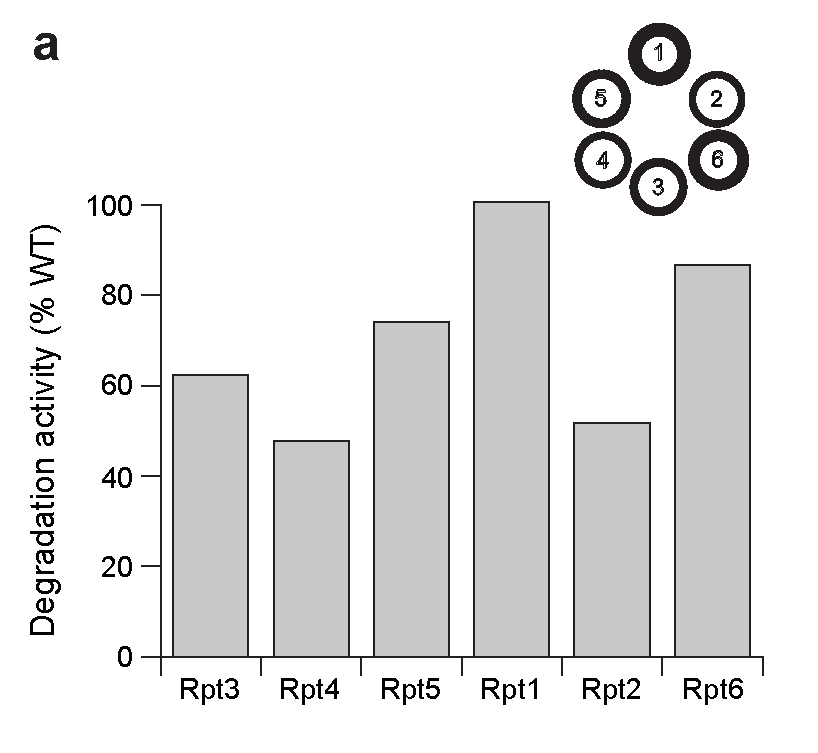
\includegraphics[scale=0.55]{pore1}
	\label{fig:pore1loops}}
\quad	
\subfigure{%
	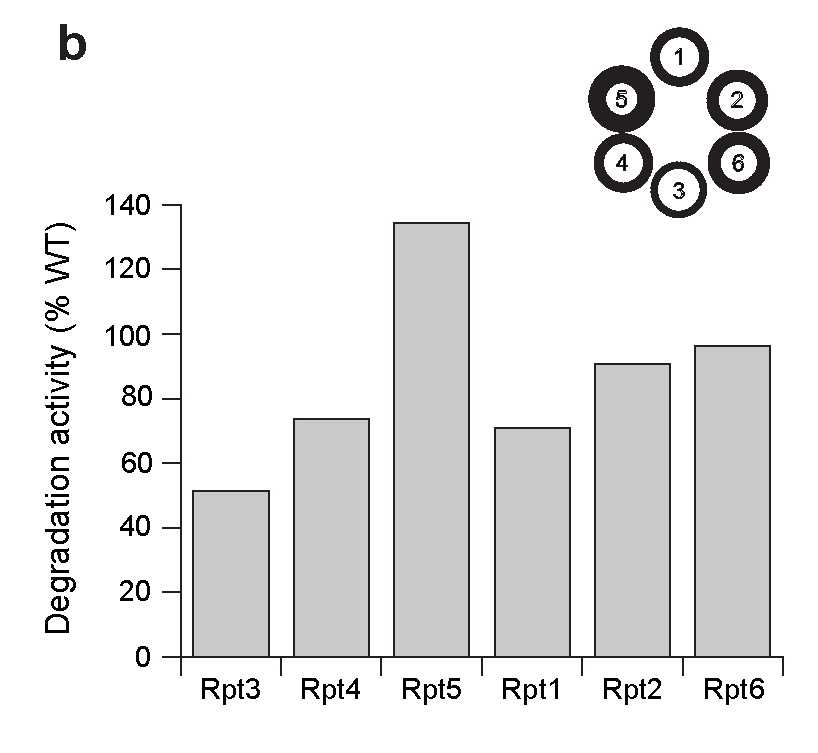
\includegraphics[scale=0.55]{pore2}
	\label{fig:pore2loops}}
%
\caption[Degradation activities for base variants containing single\--subunit pore\--loop mutations]{Degradation activities for base variants containing single\--subunit pore\--loop mutations.\par
Degradation of the polyubiquitinated GFP fusion substrate as monitored by the loss of fluorescence after addition of proteasomes reconstituted with base variants containing Y?A mutations in the Ar\--$\phi$ loops \textbf{(a)} or D?N mutations in the pore\--2 loops \textbf{(b)} of single Rpt subunits. Degradation activities under saturating conditions were measured relative to that of the reconstituted proteasome containing WT recombinant base. Errors were estimated to be $\pm$10\% (s.d.) of the mean WT value on the basis of repeat measurements (n = 3 technical replicates). The circular diagrams are alternative representations, with the line thickness corresponding to the observed degradation activities for a mutation in the respective subunit.
}
\label{fig:poreloops}
\end{figure}
%%-------------------------

All Ar\--$\phi$\--loop mutants exhibited peptidase\--gate opening activities at 65\--85\% of the wild\--type level, with the exception of mutant Rpt2, which had 38\% activity (Table~\ref{table:alldata}). Rpt2 occupies the lowest position in the apo staircase of ATPases, and docking the PAN crystal structure into the Rpt2 EM density indicates that its Ar\--$\phi$ loop is located close to the core\--particle interface, where direct or indirect contacts with the N\--termini of $\alpha$\--subunits may affect gating. However, despite this defect in gate\--opening activity, the Ar\--$\phi$\--loop mutation in Rpt2 did not lower the base affinity for the core particle (K$_D$ = 138 nM versus K$_D$ = 127 nM for wild\--type base).

Proteasomes reconstituted with the Ar\--$\phi$ mutant base variants degraded substrate at substantially different rates (Figure \ref{fig:pore1loops}). The biggest defects were observed for mutations in Rpt4 and Rpt2, which are localized clockwise\--next to the top subunit in the substrate\--free and substrate\--engaged spiral staircase, respectively. That the ranking of defects for Ar\--$\phi$-loop mutations appears shifted clockwise by one subunit relative to the defects observed for Walker\--B mutants likely results from the fact that loop mutations primarily act in cis on a subunit's ability to translocate, whereas eliminating ATP\--hydrolysis may affect conformational changes in the clockwise\--next subunits. This would be consistent with the rigid\--body model recently proposed for ClpX~\citep{Glynn2009,Glynn2012}, in which the small AAA+ subdomain of one subunit and the large AAA+ subdomain of its clockwise\--next neighbor move as one unit to propel substrate through the pore. ATP hydrolysis in a particular subunit might thus drive movements of the clockwise\--next rigid body, which includes the substrate\--interacting Ar\--$\phi$ loop of the neighboring subunit. For the proteasome, only the rigid body between Rpt3 and Rpt4 at the top of the spiral staircase appears to be present in the absence of substrate~\citep{Lander2012}, while the remaining rigid bodies form during substrate\--induced conformational changes~\citep{Matyskiela2013}. Those rigid bodies within the substrate\--engaged ATPase ring could thus cause the ranking of Rpt contributions to appear shifted by one subunit when comparing Ar\--$\phi$\--loop and Walker\--B mutants.\par

Our data qualitatively coincide with results from a recent study using endogenous 26S proteasomes from yeast, demonstrating a comparable ranking of degradation defects for individual Ar\--$\phi$\--loop mutations~\citep{Erales2012}, with the exception of Rpt2. The fact that no single Ar\--$\phi$\--loop mutation completely abrogated degradation may indicate that multiple Rpts simultaneously interact with substrate during engagement and translocation, as suggested for the bacterial unfoldase ClpX~\citep{Martin2008a}. Furthermore, removal of the Ar\--$\phi$\--loop tyrosine may not fully abolish pore\--loop function and thus cause much weaker defects than a Walker\--B mutation, which traps the entire subunit in a static ATP\--bound state. \par

The pore\--2 loop, located below the Ar\--$\phi$ loop in the central channel and directly adjacent to the Walker\--B motif, has been implicated in substrate binding and unfolding as well as peptidase interaction and the control of ATPase activity in ClpX~\citep{Martin2007,Martin2008b,Glynn2009}. A recent study on the archaeal homohexameric unfoldases Cdc48 and PAN suggested that the pore\--2 loop also interacts with the proteasomal core particle~\citep{Barthelme2013}. As the importance of the pore\--2 loop for 26S\--proteasome function is still unknown, we replaced the highly conserved aspartate with asparagine (DN) in the pore\--2 loops of individual Rpts, with Rpt2 requiring a glutamate to asparagine mutation in this position. Base variants with a single pore\--2\--loop mutation hydrolyzed ATP up to three\--fold faster than wild type, with the exception of Rpt1, which showed a 25\% decrease (Table~\ref{table:alldata}). The increased ATPase rates are reminiscent of previous observations for ClpX49 and may result from induced structural changes in the pore\--2 loop that affect the adjacent Walker\--B portion of the ATPase active site. Proteasomes reconstituted with pore\--2\--loop mutants exhibited a wide range of degradation rates (Figure \ref{pore2loops}), with the most severe defect observed for Rpt3, located at the top of the substrate\--free staircase. Changes in substrate degradation did not directly correlate with changes in ATP hydrolysis, indicating that, similar to our observations for the Ar\--$\phi$ loop, pore\--2\--loop mutations may interfere with substrate interactions and thus result in futile ATP\--hydrolysis events. The largest discrepancies between ATPase and degradation activities were observed for pore\--2\--loop mutations in Rpt3 and Rpt4, corroborating that Rpt subunits at the top of the pre\--engaged staircase are particularly important for substrate processing, presumably by enabling efficient engagement. The degradation defects do not appear to be a consequence of compromised gate opening, as all pore\--2\--loop mutants show robust peptidase\--gate opening activity, ranging from 84\% to 192\% compared to wild\--type base (Table~\ref{table:alldata}). The substantial variations in gate opening indicate that pore\--2 loops are involved in unfoldase\--peptidase communication and the Rpt C\--terminal tails are not the sole determinants of the interaction between these subcomplexes. Our results thus further emphasize the functional differences between individual Rpts. 

\subsection{HbYX\--containing C\--terminal ATPase tails mediate both peptidase binding and gate opening}
%fig nt pepstim and deg
%table NT
%fig titrations
%table KDs
%fig pulldowns

In contrast to the half\--ring asymmetry of individual Rpt contributions to substrate degradation, previous studies suggested a three\--fold symmetry for the base\--core interaction, in which the C\--terminal tails of Rpt2, Rpt3, and Rpt5 dock into core\--particle pockets~\citep{Beck2012,Lander2012}. Only these subunits contain the conserved C\--terminal HbYX (hydrophobic/tyrosine/unspecified) motif that is critical for inducing core\--particle gate opening~\citep{Smith2007,Gillette2008,Kim2011} The three remaining tails have been postulated to stabilize the complex~\citep{Smith2007}, but recent crosslinking, structural, and biochemical studies provided further conflicting results on which C\--terminal tails mediate core\--particle binding~\citep{Tian2011,Lander2012,Matyskiela2013,Park2013}. Moreover, it has been suggested that the nucleotide state of a Rpt subunit affects the conformation of its C\--terminal tail, thereby modulating peptidase interaction~\citep{Smith2011}. Individual Rpt subunits are thus expected to contribute differently to base\--core interactions, but a detailed model for the specialized roles of C\--terminal tails in peptidase binding, gate opening, and substrate transfer is lacking.\par

%%-------------------------
\begin{figure}[t!]
\centering
\subfigure{%
	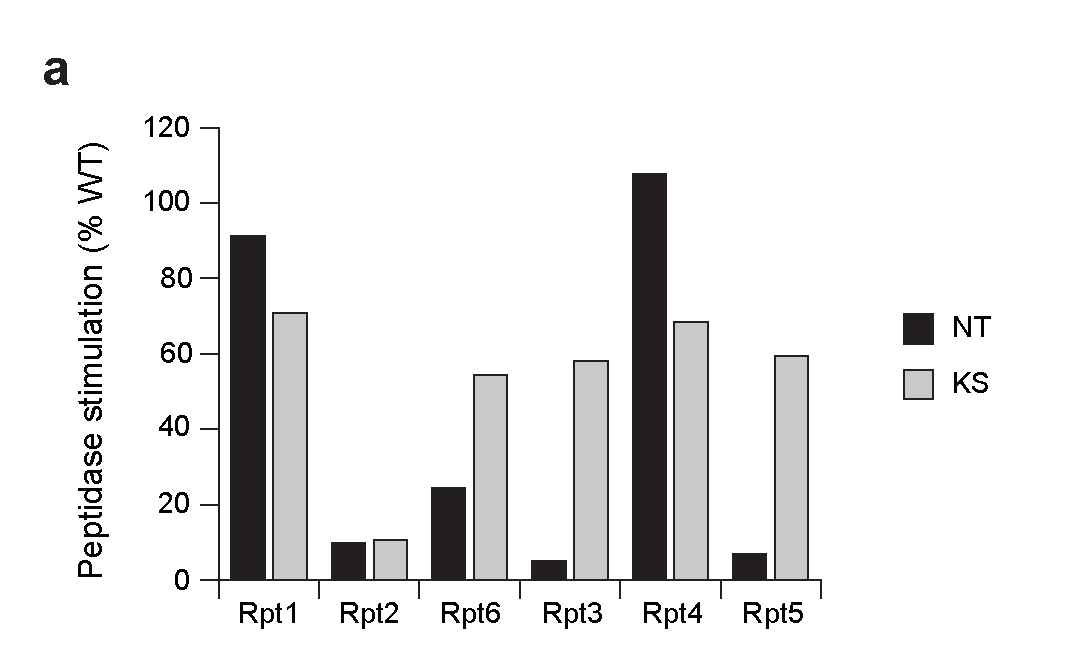
\includegraphics[scale=0.55]{tailWApepstim}
	\label{fig:tailwapepstim}}
\quad	
\subfigure{%
	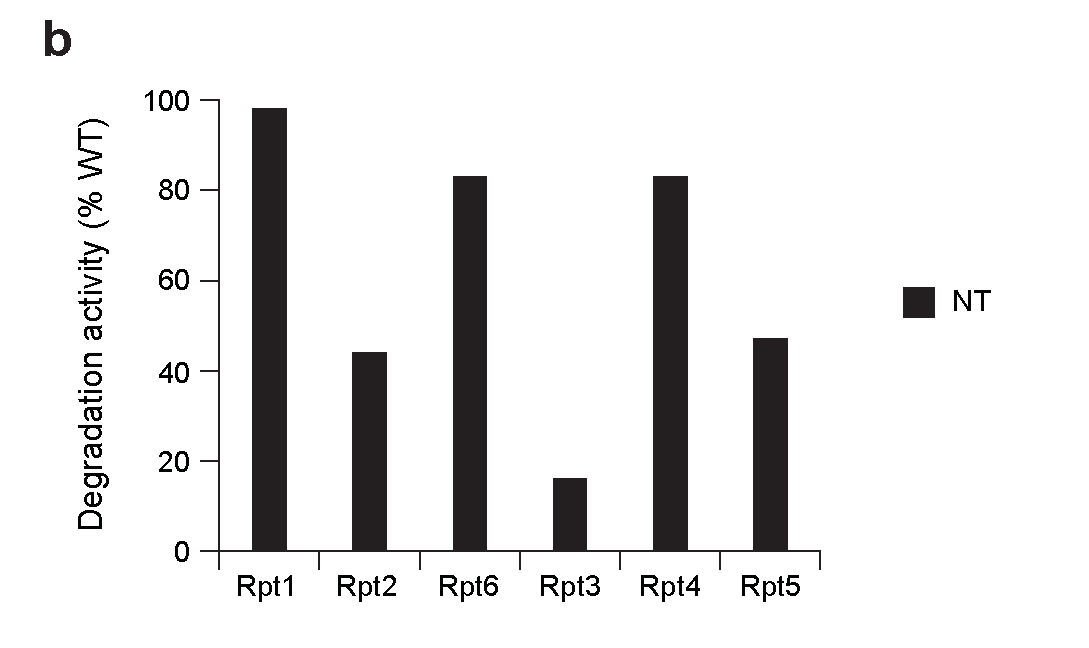
\includegraphics[scale=0.55]{taildeg}
	\label{fig:taildeg}}
%
\caption[title]{title.\par
caption.
}
\label{fig:tails}
\end{figure}
%%-------------------------


Our recombinant expression and \textit{in\--vitro} reconstitution system allows truncation of the Rpt C\--terminal tails to quantitatively characterize their contributions to stability and function of the base\--core complex. Consistent with previous studies, we found that the HbYX\--containing tails of Rpt2, Rpt3, and Rpt5 were crucial for gate opening of the core particle. These three tails were independently and nearly equally important, as their individual truncation reduced gate\--opening activity of the base by 90\--95\% (Fig. 5a, Table~\ref{table:alldata}). Surprisingly, removing the tail from Rpt6, which lacks an HbYX motif, also decreased gate opening by 75\%, whereas truncating Rpt1 and Rpt4 had little effect. \par

Titration experiments revealed that the C\--terminal tails of Rpt1, Rpt4, and Rpt6 do not contribute to the stability of the base\--core complex. The three individual tailless mutants and the triple mutant bound to core particle with K$_{D}$ values similar to or even lower than the wild\--type value (Fig. 6), which may indicate that those tails cause steric clashes or compete with neighboring HbYX\--containing tails for designated binding pockets. In contrast, truncating HbYX tails strongly affected peptidase binding. Tail truncations in Rpt2 and Rpt5 lowered the affinity for peptidase approximately 1.3\--fold and 5.6\--fold, respectively. Base lacking all three HbYX tails did not bind the peptidase (Fig. 6j). Affinity measurements for the base with tailless Rpt3 were impeded by the lack of a quantitative readout, as this mutant neither triggered core\--gate opening nor exhibited core\--mediated repression of ATPase activity.\par

%%-------------------------
\begin{figure}[b!]
\centering
\setlength{\fboxrule}{0pt}
\fbox{%
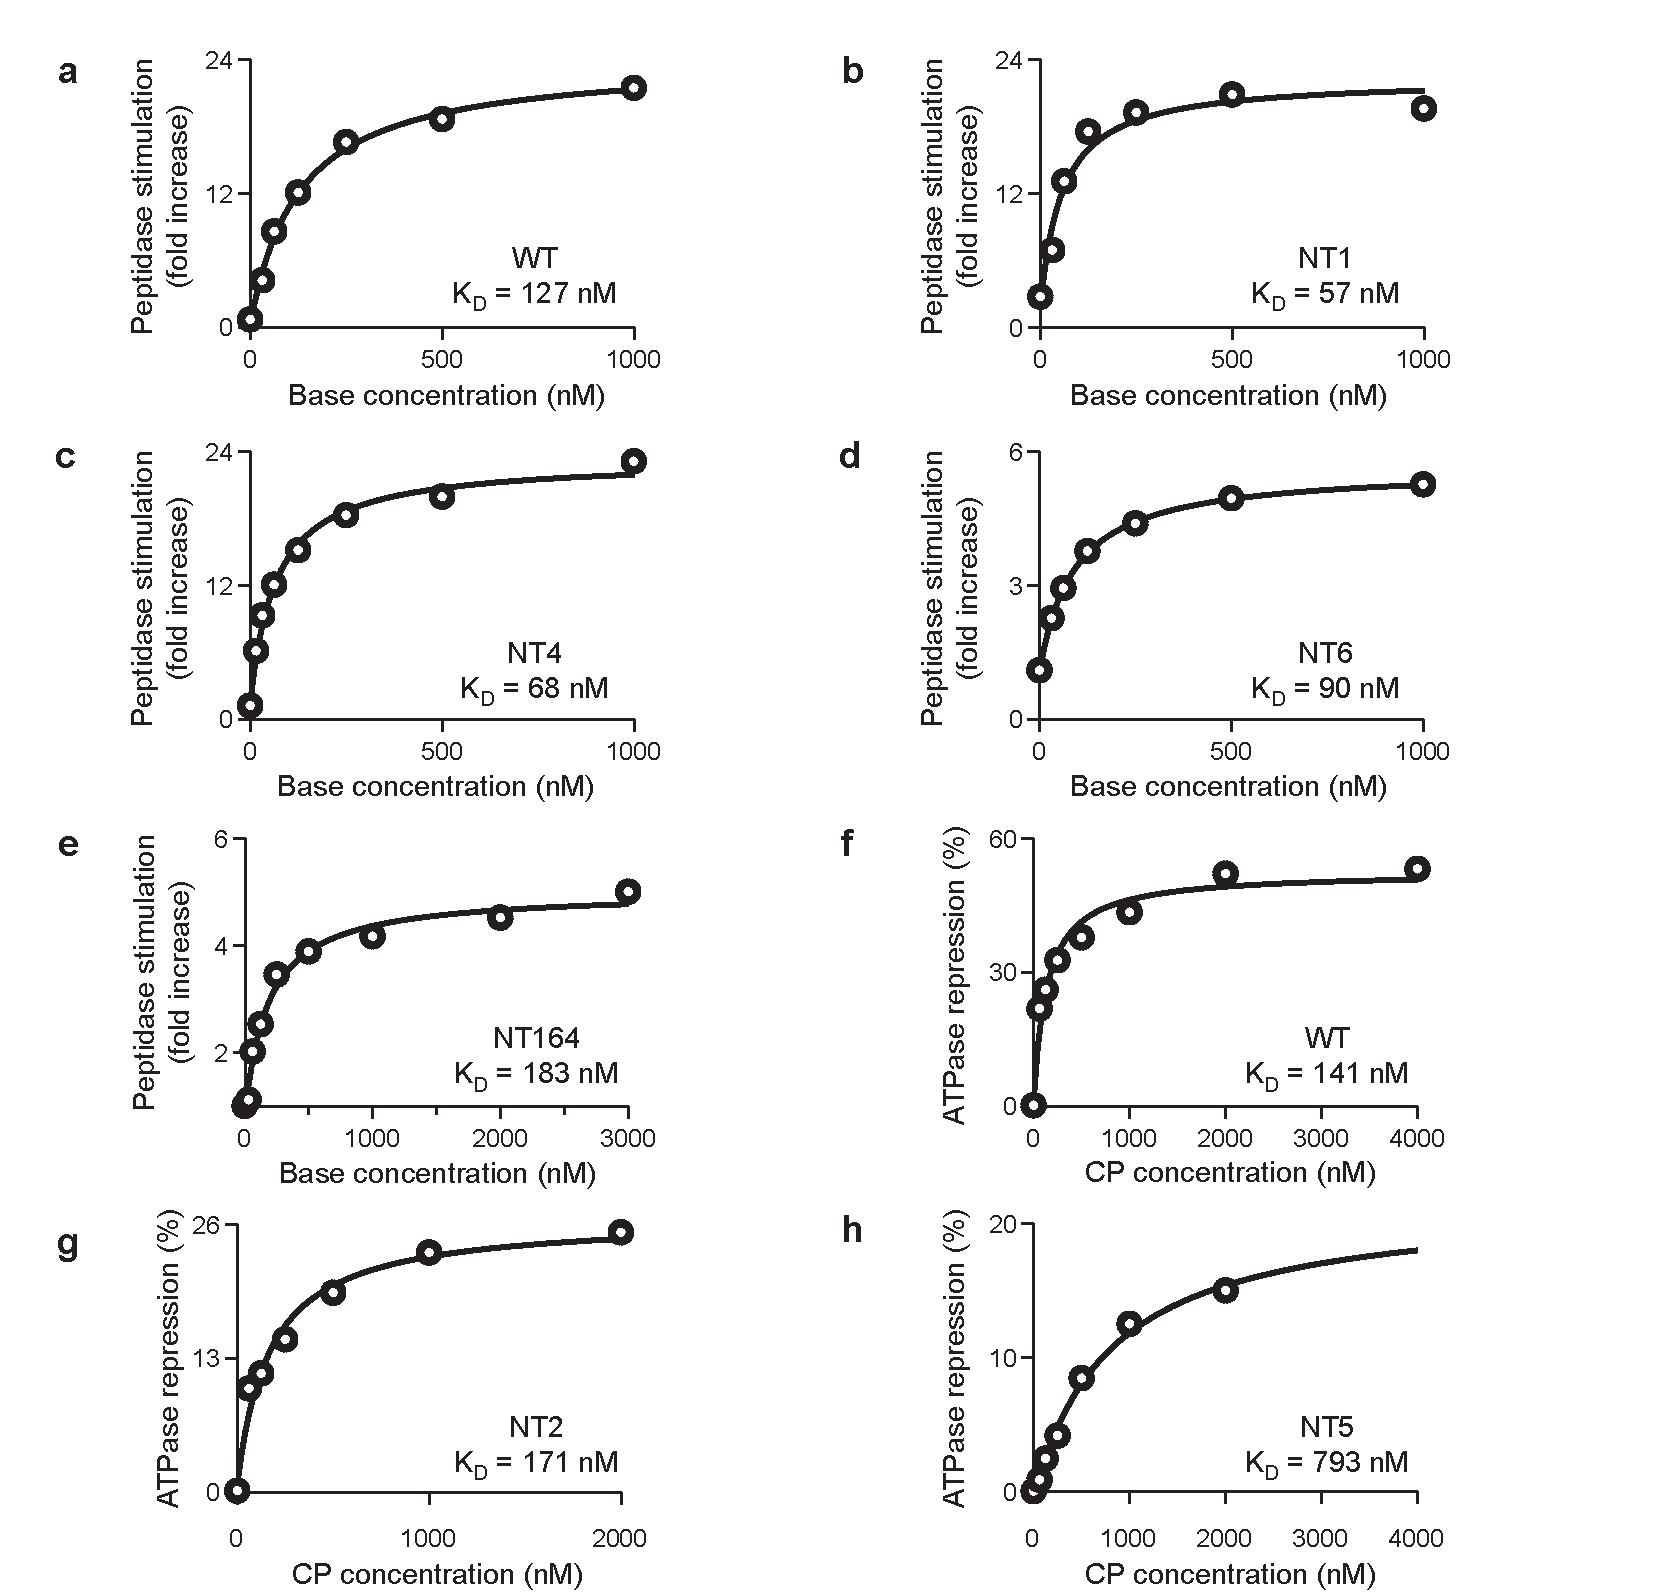
\includegraphics[scale=.55]{affinitycurves}% 
}
\caption[title]{title.\par
cation. 
}
\label{fig:tailaffinity}
\end{figure}
%%-------------------------


Proteasomes reconstituted with saturating amounts of base lacking a single tail from Rpt2, Rpt3, or Rpt5 showed decreased substrate degradation at 44\%, 16\%, or 47\% of the wild\--type rate (Fig. 5b), which is likely a consequence of gate\--opening defects. Base with tailless Rpt6 supported degradation at greater than 80\% of the wild\--type rate. Robust degradation despite compromised gate\--opening activity, as observed for Rpt6, may occur because translocation by the base pushes substrate through a partially opened gate, whereas the gate\--opening assay reports solely on peptide diffusion into the peptidase.

%%-------------------------
\begin{figure}[h!]
\centering
\setlength{\fboxrule}{0pt}
\fbox{%
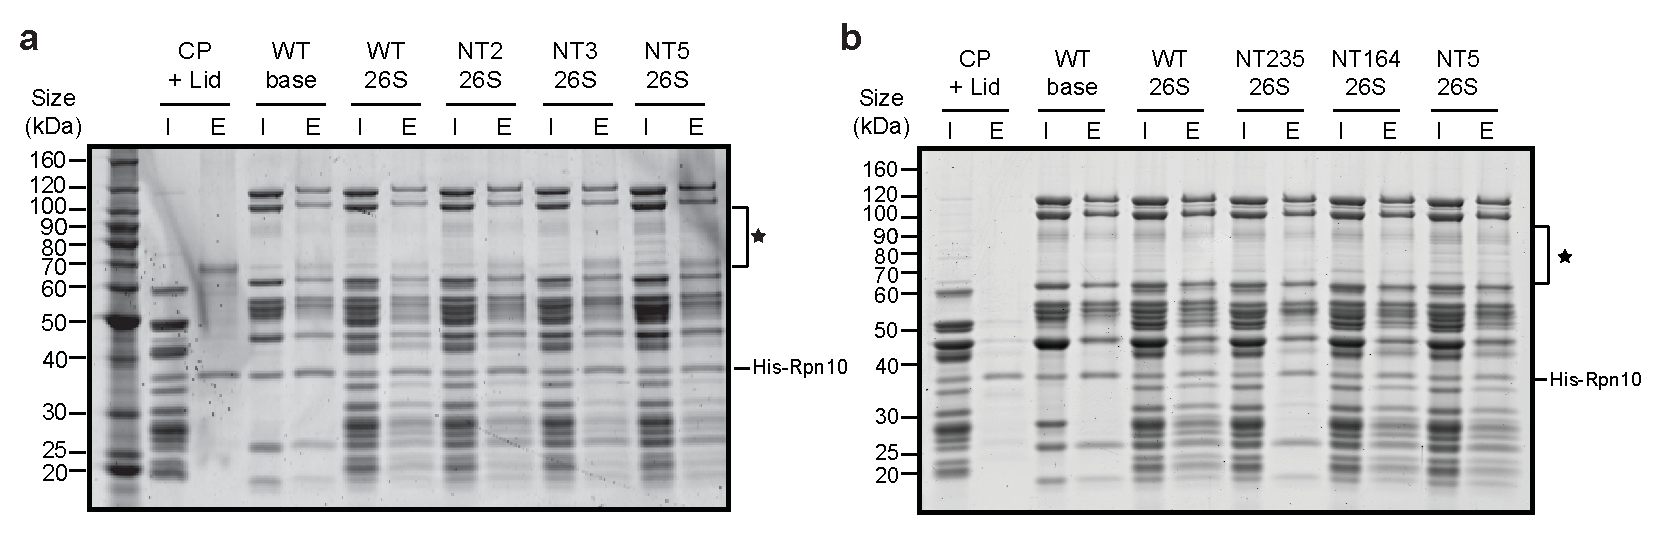
\includegraphics[scale=.55]{ntpulldowns}% 
}
\caption[title]{title.\par
cation. 
}
\label{fig:ntpulldowns}	
\end{figure}
%%-------------------------

\subsection{Individual ATPase tails modulate peptidase gate opening in a nucleotide\--independent manner}
%fig wa ks deg
%table WA
Interaction of base and core particle to open the gate is known to be ATP\--dependent and differentially stimulated by various ATP\--analogs~\citep{Smith2005,Liu2006,Li2009}. It has been postulated for some homohexameric unfoldases, including PAN and HslU, that ATP hydrolysis may drive conformational changes in the C\--terminal tails of individual subunits and thereby regulate nucleotide\--dependent binding and gating interactions with the peptidase~\citep{Seong2002,Smith2005,Smith2007}. Based on this model, an ATP\--bound subunit would have an exposed C\--terminal tail that interacts with the core particle, whereas an empty\-- or ADP\--state subunit would have its tail buried in an occluded conformation. It was further proposed that at any given time the 26S proteasome has only two Rpt subunits, arranged in para position across the ring, in an ATP\--bound state with C\--terminal tails exposed for peptidase interaction~citep{Smith2011}. \par

We tested whether peptidase interaction of an Rpt tail in fact depends on the nucleotide state of the particular subunit. According to this model, removing a given tail should resemble trapping that subunit in an empty\--state conformation. We therefore prevented nucleotide binding to individual Rpts by mutating the conserved lysine to serine (KS) in their Walker\--A motifs (see \ref{methods:mutations}). We produced base variants with single\--subunit KS mutations and found that only mutation of Rpt2 caused severe base\--assembly defects. Characterization of the other KS mutants demonstrated that trapping a particular Rpt subunit in an empty state has much weaker effects on gate\--opening activity than truncating its C\--terminal tail (Fig. 5a). Base containing a KS mutation in Rpt3 or Rpt5 retained 58\% or 59\% of wild\--type gate\--opening activity, whereas the corresponding tailless mutants showed only 5\% or 7\% activity. Trapping Rpt6 in an empty state preserved 54\% of wild\--type activity, whereas removing its tail reduced gate opening to 25\%. Moreover, all base variants with single KS mutations exhibited some degree of misassembly, such that the measured gate\--opening activities represent only lower bounds. Thus, contrary to previous models, the C\--terminal tails are accessible for peptidase binding independent of the nucleotide state of individual Rpt subunits, even though the base\--core interaction depends on a global ATP\--bound conformation of the Rpt ring. \par

The Walker\--A mutants were not suited to qualitatively analyze the contribution of individual Rpt subunits to substrate processing as they caused universally severe degradation defects (Table~\ref{table:alldata}). In contrast to fixing subunits in an ATP\--bound state with a Walker\--B mutation, empty\--state subunits potentially influence the hexamer conformation or compromise subunit communication required for processive ATP\--hydrolysis in the ring.

%-----------------------------
\newpage
\vfill

\begin{table}[H]
\footnotesize
\centering
\ra{1.3}
\caption[Biochemical characterization of reconstituted 26 proteasome base mutants]{Biochemical characterization of reconstituted 26 proteasome base mutants.}
\begin{tabular*}{1\textwidth}{@{}lcccccccccc@{}}\toprule
& \multicolumn{1}{C{1.5cm}}{Mutated Residue} & \phantom{} & \multicolumn{2}{C{2.9cm}}{basal ATPase rate} & \phantom{} & \multicolumn{2}{C{3.8cm}}{peptidase stimulation} & \phantom{} & \multicolumn{2}{C{4cm}}{degradation rate (k$_{deg}$)}\\
\cmidrule{2-2} \cmidrule{4-5} \cmidrule{7-8} \cmidrule{10-11}
 & & & min$^{\--1}$ & \% WT & & fold increase & \% WT & & (enz$^{\--1}$ min$^{\--1}$) & \% WT\\ \midrule

Holoenzyme & \-- & & 107 & \-- & & \-- & \-- & & $0.32$ & \--\\
WT (\textit{E. coli}) & \-- & & 51 & 100 & & 21 & 100 & & 0.30 & 100\\
WT (yeast) & \-- & & 54 & 106 & & 22 & 103 & & 0.29 & 97\\
E$\rightarrow$Q hexamer	& \-- & & 2 & 4 & & 24 & 110 & & 0.00 & 0.00\\
EQ1 & 310 & & 35 & 68 & & 15 & 68 & & 0.08/0.12 & 27/40\\
EQ2 & 284 & & 82 & 161 & & 29 & 134 & & 0.28/0.24 & 92/79\\
EQ3 & 273 & & 17 & 33 & & 19 & 89 & & 0.005/0.00 & 2/0\\
EQ4 & 282 & & 55 & 108 & & 20 & 95 & & 0.001/0.00 & 0.41/0\\
EQ5 & 282 & & 34 & 67 & &  25 & 118 & & 0.13/0.21 & 44/72\\
EQ6 & 249 & & 83 & 164 & &  35 & 161 & & 0.02/0.01 & 6/5\\
YA1 & 284 & & 66 & 129 & & 18 & 84 & & 0.30 & 101\\
YA2 & 257 & & 75 & 148 & &  8 & 38 & &  0.15 & 52\\
YA3 & 246 & & 44 & 87 & & 17 & 81 & &  0.19 & 62\\
YA4 & 255 & & 38 & 75 & & 14 & 65 & &  0.16 & 54\\
YA5 & 255 & & 89 & 174 & & 15 & 68 & &  0.22 & 74\\
YA6 & 222 & & 38 & 76 & & 18 & 82 & &  0.26 & 87\\
DN1 & 327 & & 39 & 76 & & 23 & 106 & &  0.21 & 71\\
EN2 & 300 & & 59 & 115 & & 24 & 110 & &  0.27 & 91\\
DN3 & 289 & & 65 & 127 & & 20 & 91 & &  0.16 & 52\\
DN4 & 298 & & 141 & 278 & & 41 & 192 & &  0.22 & 74\\
DN5 & 298 & & 90 & 177 & & 32 & 149 & &  0.40 & 134\\
DN6 & 265 & & 58 & 113 & & 18 & 84 & &  0.29 & 96\\
NT1 & 464\--468 & & 61 & 121 & & 20 & 91 & & 0.29 & 98\\
NT2 & 434\--438 & & 45 & 88 & & 2 & 10 & & 0.13 & 44\\
NT3 & 424\--428 & & 65 & 127 & & 1 & 5 & & 0.05 & 16\\
NT4 & 433\--437 & & 49 & 97 & & 23 & 108 & & 0.25 & 83\\
NT5 & 430\--434 & & 86 & 169 & & 1 & 7 & & 0.14 & 47\\
NT6 & 401\--405 & & 53 & 104 & & 5 & 24 & & 0.25 & 83\\
KS1 & 257 & & 32$^a$ & 62$^a$ & & 15 & 71 & & 0.07$^a$ & 24$^a$\\
KS2 & 230 & & 13$^a$ & 25$^a$ & & 2 & 10 & & ND$^a$ & ND$^a$\\
KS3 & 219 & & 29$^a$ & 57$^a$ & & 12 & 58 & & 0.08$^a$ & 26$^a$\\
KS4 & 228 & & 15$^a$ & 29$^a$ & & 15 & 68 & & 0.001$^a$ & 0.40$^a$\\
KS5 & 228 & & 74$^a$ & 147$^a$ & & 13 & 59 & & 0.02$^a$ & 6$^a$\\
KS6 & 195 & & 22$^a$ & 43$^a$ & & 12 & 54 & & 0.04$^a$ & 15$^a$\\

\bottomrule
\end{tabular*}
\label{table:alldata}
\end{table}
%-----------------------------




%%-------------------------

\section{Discussion}
%fig model

Our mutational studies using heterologously expressed base subcomplex and \textit{in\--vitro} reconstituted 26S holoenzymes revealed that substrate degradation by the proteasome relies on distinct functional asymmetries with strongly non\--equivalent contributions of individual Rpts. While a static three\--fold symmetry determines the interactions between the base ATPase ring and the core particle, substrate degradation seems to depend on asymmetric spiral\--staircase arrangements of the ATPases in which subunits close to the pore entrance play crucial roles in substrate engagement (Fig. 7). \par

Our data demonstrate a clear three\--fold symmetry at the base\--core interface, in which the HbYX\--containing C\--terminal tails of the alternating subunits Rpt2, Rpt3, and Rpt5 are critical for both binding the core particle and triggering gate opening (Fig. 7). The tails of the interjacent Rpt1, Rpt4, and Rpt6 are dispensable for the base\--peptidase interaction, and Rpt1 and Rpt4 are largely irrelevant for gate opening. The apparent function of the Rpt6 tail in core\--particle gating may result from Rpt6's role in ensuring the correct register of the heterohexameric base atop the $\alpha$\--ring of the core particle. Recent structural and functional data suggest that Rpt6 plays a role in base\--core assembly and its C\--terminus is the only non\--HbYX tail that docks into just one specific $\alpha$ pocket~\citep{Tian2011,Park2013}. It is thus possible that Rpt6's tail prevents the neighboring HbYX\--containing tails from mispairing with this pocket. \par

Interactions of the three HbYX\--containing tails with the peptidase seem static and independent of the nucleotide state of the particular Rpt subunits. This finding contradicts previous models proposing that the Rpt C\--terminal tails change conformation during the ATP\--hydrolysis cycle and thus lead to a ``wobbling'' of the base atop the peptidase~\citep{Smith2005,Smith2007,Smith2011}. Earlier structural studies demonstrated that in the absence of ATP several AAA+ hexamers adopt a ``lockwasher'' conformation~\citep{Singleton2000,Guo2002,Kim2003} that likely prevents binding to the planar surface of a peptidase. The ATP\--dependence of the base\--core interaction thus seems to originate not from conformational changes of individual tails, but rather from the global geometry of the ATPase ring, which must be at least partially nucleotide\--bound to facilitate peptidase docking. \par

Eliminating ATP hydrolysis or introducing Ar\--$\phi$\--loop mutations in single Rpts revealed that the lid\--facing half of the ATPase ring is particularly crucial for substrate degradation. These key Rpts occupy top positions in the spiral\--staircase arrangement adopted by the large AAA+ subdomains in the absence of substrate (Fig. 7), and they must undergo ATP\--hydrolysis\--induced conformational changes to engage an incoming substrate and initiate translocation. The Rpt hexamer then transitions to an alternative, more planar staircase arrangement, in which Rpt1 occupies the top position and rigid\--body interfaces are formed between most subunits~\citep{Matyskiela2013}. Our data suggest that ATP hydrolysis in Rpt1 is more important than in neighboring subunits to drive substrate translocation, possibly because Rpt1 triggers a burst of coordinated hydrolysis events around the ring. Nevertheless, individual Rpts may contribute more equally to translocation once substrate is engaged. \par

%%-------------------------
\begin{figure}[b!]
\centering
\setlength{\fboxrule}{0pt}
\fbox{%
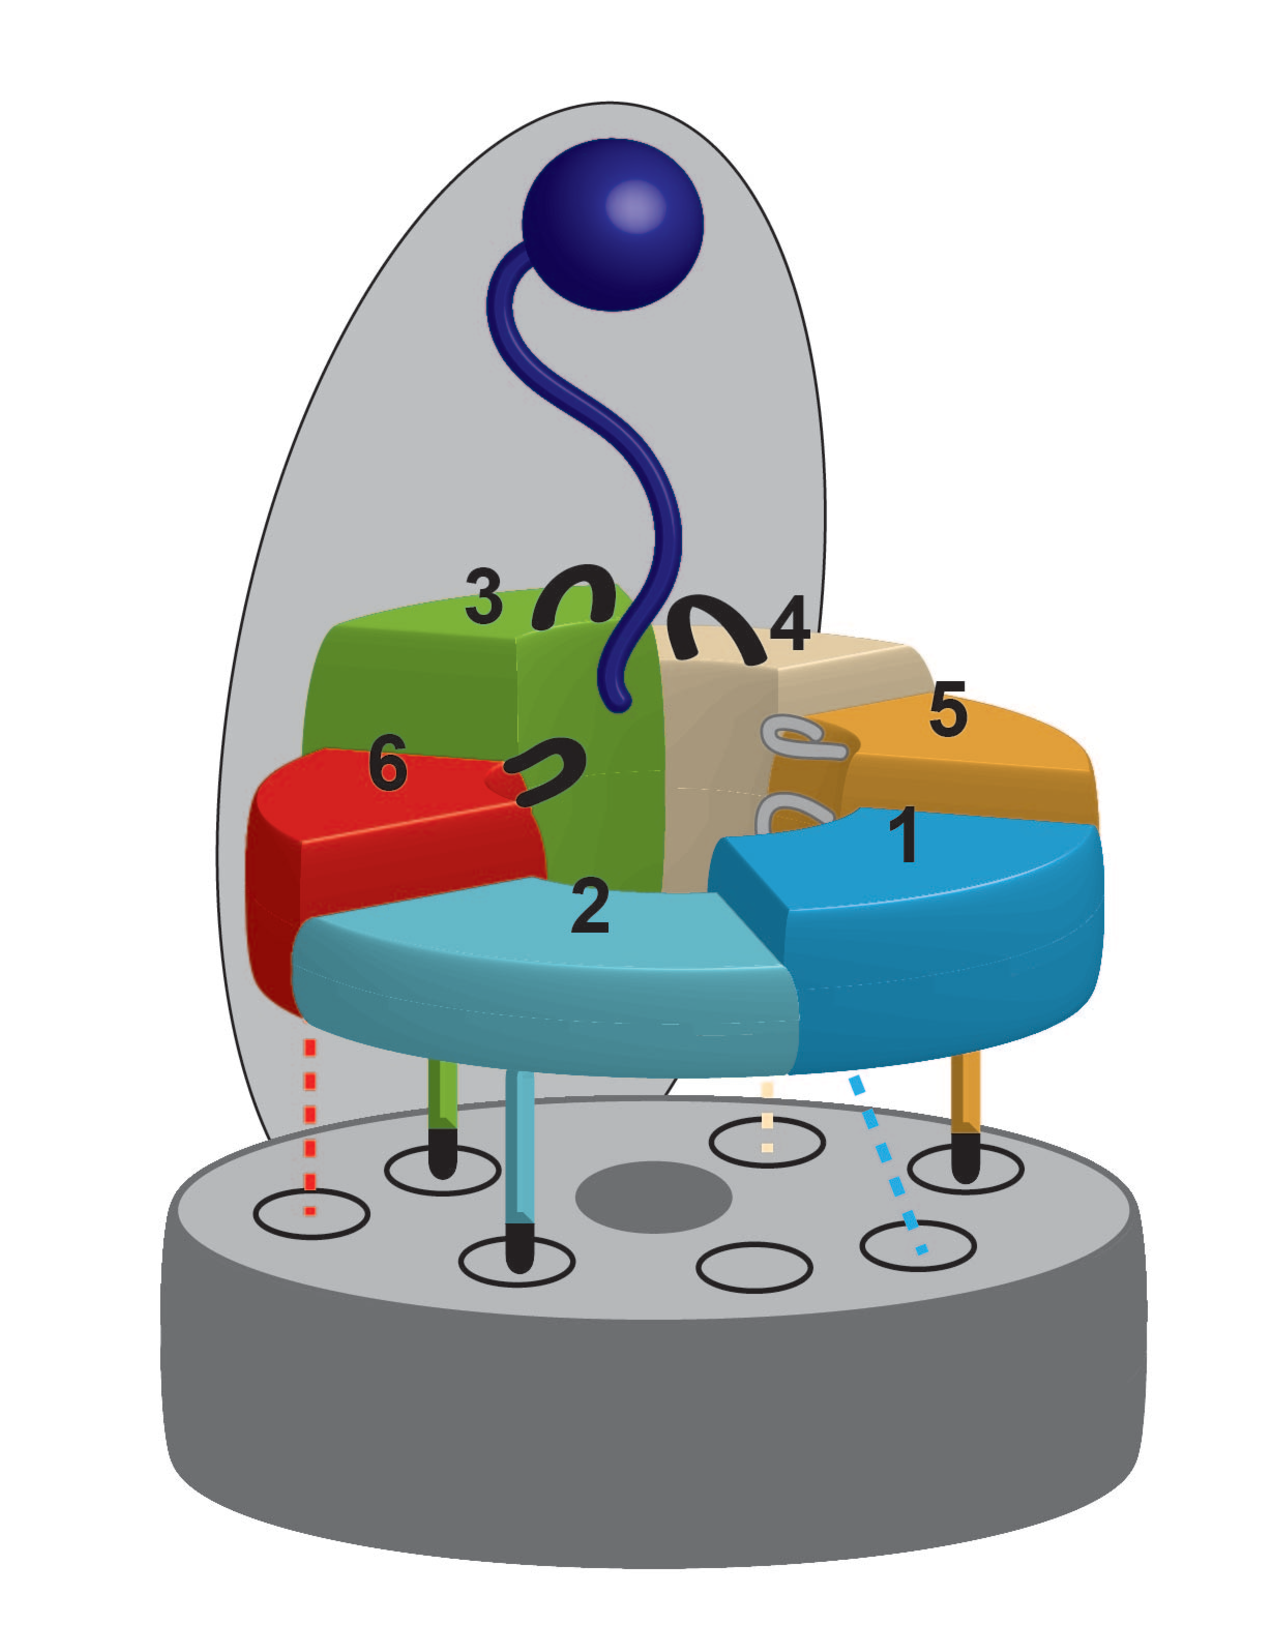
\includegraphics[scale=.55]{model}% 
}
\caption[title]{title.\par
cation. 
}
\label{fig:model}	
\end{figure}
%%-------------------------

Spiral\--staircase arrangements have been previously observed in several homohexameric motors of the AAA+ and RecA families, and it has been suggested that individual ATPase subunits successively transition through the different vertical registers of the spiral to drive substrate translocation~\citep{Singleton2000,Enemark2006,Glynn2009,Thomsen2009,Costa2011}. However, the apparently rigid spiral\--staircase configurations observed for the proteasomal ATPase ring in the absence and presence of substrate, together with the biochemical data presented here, contradict stepwise successive progression of individual Rpts through the different registers. Instead, the proteasome base relies on differential subunit contributions prescribed by the regulatory particle's asymmetric architecture. Conformational changes in the top subunits of a pre\--engaged staircase thread an incoming substrate, before the ATPase ring switches to an engaged staircase arrangement, in which subunits contribute more equally to protein translocation. \par

Although all mutant base complexes in this study were characterized by \textit{in\--vitro} assays that may or may not wholly recapitulate the complexity of \textit{in\--vivo} conditions, our results agree with and substantially extend earlier findings, suggesting non\--equivalent contributions of individual Rpt subunits to substrate processing by the 26S proteasome~\citep{Rubin1998,Erales2012,Kim2012}. Protein degradation by the proteasome deviates from models previously proposed for other AAA+ unfoldases, pointing toward major differences between the operating principles of homo\-- and heterohexameric AAA+ motors. Future experiments will have to address to what extent these motor designs rely on different strategies for substrate engagement, generation of mechanical force for unfolding, and translocation of the polypeptide chain into a peptidase for degradation.

%%-------------------------

\section{Materials and Methods}

\subsection{Base mutagenesis and purification of base complexes}
Point mutations in individual ATPase subunits were generated by PCR using pETDuet\--1 plasmids containing individual Rpt subunits, which were then used for amplification and substitution into the wild type hexamer in pCOLADuet\--1. Base expression strains were generated by co\--transforming the pETDuet\--1, pCOLA\--1 and pACYCDuet\--1 plasmids into \textit{E. coli} BL21\--star (DE3) cells. The base subcomplex was produced by growing the expression strain to OD$_{600}$=0.6\--0.8 and inducing with 1 mM isopropyl\--b\--D\--thiogalactopyranoside overnight at 18�C. Cells were harvested by centrifugation at 5000 rpm for 15 minutes, resuspended in nickel buffer (25 mM HEPES pH 7.6, 100 mM NaCl, 100 mM KCl, 10 \% glycerol, 10 mM MgCl$_{2}$, 0.5 mM EDTA, 20 mM imidazole) supplemented with 2 mg ml$^{-1}$ lysozyme, protease inhibitors and benzonase. Cells were lysed by freeze\--thaw and sonication on ice for 1 minute 30 seconds in 15 second bursts. Lysate was clarified by centrifugation at 15,000 rpm at 4�C for 30 minutes. A two\--step affinity purification of the base subcomplex was performed using Ni\--NTA agarose (Qiagen) to select for His$_6$\--Rpt3 and anti-FLAG M2 resin (Sigma-Aldrich) selecting for FLAG\--Rpt1. 0.5 mM ATP was present in all purification buffers. The Ni\--NTA and anti\--FLAG M2 columns were eluted with nickel buffer containing 250 mM imidazole or 0.15 mg ml$^{-1}$ 3xFLAG peptide, respectively. The Flag column eluate was concentrated using a 30,000 MWCO concentrator (Amicon) and run on a Superose 6 gel filtration column (GE Healthcare) equilibrated with gel filtration buffer (60 mM HEPES pH 7.6, 50 mM NaCl, 50 mM KCl, 10 \% glycerol, 5 mM MgCl$_{2}$, 0.5 mM EDTA, 1 mM DTT, 0.5 mM ATP).

\subsection{Mutation of conserved AAA+ motifs}\label{methods:mutations}
%fig sequence alignment
%results various WB and WA mutations

To fix subunits in a constitutively ``ATP\--bound'' state~\citep{Hanson2005}, we examined mutations in the conserved Walker-B glutamate-aspartate motif by placing the same mutation in all six Rpt subunits simultaneously and characterizing the functional activities of the mutant base hexamers. We constructed a series of mutant hexamers containing single mutations of glutamate to glutamine (DN) or aspartate to asparagine (EQ) as well as the double DN EQ mutant. Rpt subunits carrying the DN mutation assembled properly into a hexamer that lacked ATPase activity. However, the DN mutation also had undesired deleterious effects, as this base variant was deficient in peptidase gate opening, even though a permanently ATP\--bound hexamer is expected to interact with and maximally stimulate the core particle. The DN EQ double mutation resulted in an even stronger defect and prevented assembly of the ATPase hexamer, as indicated by the lack of an appropriate elution peak in size exclusion chromatography (unpublished data, R.B.).  The EQ mutation supported proper base assembly, eluted at the appropriate volume from a size exclusion column, and was deficient in ATPase activity yet exhibited wild-type levels of peptidase stimulation (Table~\ref{table:alldata}).  We deduced that the EQ mutation approximated an ``ATP-bound'' state and utilized this mutation for subsequent studies of the contribution of individual Rpt subunits to base activities (Figure \ref{fig:wbdeg}, Table~\ref{table:alldata}, Supplementary Fig. 4, and Supplementary Fig. 5).\par

We required an appropriate mutation to induce a permanent empty state, either by preventing the conformational response of a subunit to ATP binding or by interfering with ATP binding itself. For some AAA+ enzymes, including ClpX from \textit{E. coli}, mutation of the Sensor\--II arginine has been shown to induce an empty\--state conformation~citep{Song2000,Joshi2004,Hanson2005}, yet the proteasomal clade of classic AAA+ enzymes lacks a conserved Sensor\--II arginine. We therefore mutated the Walker A lysine to abrogate nucleotide binding altogether. First we mutated the lysine to either arginine (KR) or serine (KS) in all six Rpt subunits simultaneously to clearly establish the effects on base activity. The KR mutant hexamer exhibited activities in ATP hydrolysis and peptidase stimulation that were similar to wild\--type base (unpublished data, R.B.), indicating that the KR mutation does not interfere with ATP binding of Rpt subunits. Conversely, the KS mutation resulted in severe assembly defects that prevented us from purifying the six\--fold mutant base. This finding would be consistent with a completely empty\--state hexamer and supports previous observations that assembly of the base is ATP dependent~citep{Lee2012}. Furthermore, KS mutations in some individual Rpt subunits have been shown to interfere with cellular assembly of the 26S proteasome, compromise substrate degradation~citep{Kim2012}, and cause severe growth defects \textit{in vivo}~citep{Rubin1998}. Preventing ATP binding simultaneously in all six subunits is likely more deleterious for ring assembly than placing the KS mutation in just a single Rpt at a time, as the assembly process may require only some subunits to fill with nucleotide. We therefore placed KS mutations in single Rpt subunits and characterized the functional activities of the resulting mutant base subcomplexes (Figure~\ref{fig:tailwapepstim}, Table~\ref{table:alldata}).  Only a mutation in Rpt2 caused extreme defects in base assembly, although all base variants with single KS mutations did exhibit some degree of misassembly. 

\subsection{Purification of endogenous yeast complexes}
Yeast holoenzyme, core particle, base and lid subcomplexes were purified from \textit{S. cerevisiae} essentially as previously described~\citep{Leggett2005}. Frozen yeast cells were lysed using a Spex SamplePrep 6870 Freezer/Mill. Holoenzyme was purified from a yeast strain containing FLAG\--Rpn11. Lysed cells were resuspended in lysis buffer containing 60 mM HEPES pH 7.6, 100 mM NaCl, 100 mM KCl, 10\% glycerol, 5 mM MgCl2, 0.5 mM EDTA, 0.2\% NP\--40 and ATP regeneration mix (5 mM ATP, 0.03 mg ml$^{-1}$ creatine kinase, 16 mM creatine phosphate). Holoenzyme was bound to anti\--FLAG M2 resin and washed with wash buffer (60 mM HEPES pH 7.6, 100 mM NaCl, 100 mM KCl, 10\% glycerol, 5 mM MgCl$_2$, 0.5 mM EDTA, 0.1\% NP-40, 0.5 mM ATP). Holoenzyme was eluted with 0.15 mg ml$^{-1}$ 3xFLAG peptide and further purified by gel filtration using a Superose 6 column with gel filtration buffer (see above). Lid and base subcomplexes were isolated from FLAG\--Rpn11 or FLAG\--Rpn2 yeast strains, respectively, and purified by exposure to a 1 M NaCl wash while bound to anti\--FLAG M2 resin. Base purification buffers included 0.5 mM ATP. Core particle was purified from a 3xFLAG\--Pre1 yeast strain using a 500 mM salt wash. All subcomplexes underwent size exclusion chromatography using a Superose 6 column as described above.

\subsection{Yeast strains}
Yeast lid and holoenzyme were purified from strain YYS40 (genotype MATa ade2\--1 his3\--11,15 leu2\--3,112 trp1\--1 ura3\--1 can1 Rpn11::Rpn11\--3XFLAG(HIS3), source Y. Saeki). Core particle was prepared either from strain RJD1144 (genotype MATa his3\--200 leu2\--3,112 lys2\--801 trp\--63 ura3\--52 PRE1\--FLAG\--6xHIS::Ylpac211(URA3) source R. Deschaies) or strain yAM14 (genotype MATa ade2\--1 his3\--11,15 leu2\--3,112 trip1\--1 ura3\--1 can1\--100 bar1 PRE1::PRE1\--3XFLAG(KanMX), this work).

\subsection{ATPase and peptidase stimulation assays}
ATPase activity was quantified using an NADH\--coupled ATPase assay. 500 nM base was incubated with 1x ATPase mix (3 U ml$^{-1}$ pyruvate kinase, 3 U ml$^{-1}$ lactate dehydrogenase, 1 mM NADH, 7.5 mM phosphoenol pyruvate) at 30�C. Absorbance at 340 nm was monitored for 900 seconds at 10 second intervals using a UV\--Vis Spectrophotometer (Agilent). Peptidase stimulation was monitored by following the increase in fluorescence resulting from cleavage of a fluorogenic peptide substrate~\citep{Glickman1998}, Suc\--LLVY\--AMC (Boston Biochem), using a QuantaMaster spectrofluorimeter (PTI). 50 nM core particle was incubated with saturating base subcomplex in the presence of an ATP regeneration system (5 mM ATP, 16 mM creatine phosphate, 6 mg ml$^{-1}$ creatine phosphokinase) and 50 $\mu$M Suc-LLVY-AMC.


\subsection{ATPase repression and peptidase stimulation titrations}
Titration experiments were conducted using either 25 nM core particle and increasing amounts of base (peptidase stimulation) or 100 nM base and increasing amounts of core particle (ATPase activity). K$_{D}$ values were extracted by fits to a simple binding curve using Grafit (Erithacus Software).

\subsection{Fluorescent substrate degradation assay}
Proteasome holoenzyme was reconstituted from core particle, lid, base and Rpn10. A GFP\--titin$^{V15P}$\--cyclin\--PY fusion protein was modified \textit{in vitro} with a polyubiquitin chain using Uba1, Ubc1, Rsp5 and wild\--type ubiquitin. Degradation reactions were performed at 30�C in gel filtration buffer (60 mM HEPES pH 7.6, 50 mM NaCl, 50 mM KCl, 10 \% glycerol, 5 mM MgCl$_{2}$, 0.5 mM EDTA, 1 mM DTT, 0.5 mM ATP) supplemented with an ATP regeneration system. Single and multiple turnover degradation activities were monitored by the loss of GFP fluorescence (excitation 467 nm; emission 511 nm) using a QuantaMaster spectrofluorimeter (PTI). Multiple turnover degradation experiments were performed with 50 nM reconstituted holoenzyme under V$_{max}$ conditions (saturating base, lid and Rpn10) with 2 $\mu$M substrate. Excess base, lid, and Rpn10 did not affect the observed degradation rate (see \ref{degcontrols}). For single turnover degradation, 2 $\mu$M holoenzyme was reconstituted from equimolar concentrations of subcomplexes and mixed with 100 nM substrate. Single turnover degradation traces were best fit with double exponential decay curves using Grafit (Erithacus Software).

\subsection{Native gel electrophoresis}
Analysis of proteasome holoenzyme and subcomplexes by native gel was performed as described previously~\citep{Leggett2005}. Assembly reactions were incubated for 15 minutes at 23�C with 5 mM ATP, followed by electrophoresis on a 3.5 \% native polyacrylamide gel. Electrophoresis was conducted at 4�C with stirring and running buffer containing 0.5 mM ATP. The gel was overlaid with developer solution (running buffer with 100 nM Suc\--LLVY\--AMC peptide and 0.02 \% SDS) and incubated at 30�C for 10 minutes prior to imaging. Fluorescence imaging was performed using a Typhoon scanner (GE Healthcare) and followed by Coomassie staining.

\subsection{Affinity pulldowns}
Base subcomplexes were mixed with core particle, lid and Rpn10 in nickel buffer with 1x ATP regeneration system at 23�C for 15 minutes. All components were present at a concentration of 900 nM in the reaction, which was then incubated with 5 $\mu$l of magnetic Dynabeads (Invitrogen) at 23�C for 15 minutes. The beads were washed three times with nickel buffer supplemented with 0.05 \% NP-40 and 0.5 mM ATP. Bound proteins were eluted with nickel buffer containing 500 mM imidazole. Pulldown samples were run on a 10 \% SDS-PAGE gel, stained with Sypro Ruby and imaged using a Typhoon scanner (GE Healthcare).



%%-------------------------



% Chapter 4

\chapter{Substrate engagement and subunit communication} % Write in your own chapter title
\label{Chapter4}
\lhead{Chapter 4. \emph{Substrate engagement and subunit communication}} % Write in your own chapter title to set the page header


\section{Introduction}

%%-------------------------

\section{Results}

\subsection{Monitoring substrate engagement by the base unfoldase}
%fig titin concatemers and reaction schematic
%ub?
%scans
%MTO
%STO with curve fits and rate constants

%fig DATA

Data, as seen in Figure \ref{fig:titinconstructs} and Figure \ref{fig:titintablegel}.

And schematic and chemical structure in Figure \ref{fig:reactionscheme} and Figure \ref{fig:titinstructure}.

More data, as seen in Figure \ref{fig:titincarboxy}.

%\begin{table}[H]
	%\centering
%	\ra{1.3}
%	\caption[Titin concatamer molecular weights]{Titin concatamer molecular weights.}
%\begin{tabular*}{.5\linewidth}{ m{0.15\linewidth}C{0.15\linewidth} C{0.15\linewidth} }\toprule
%Construct & Number of Amino Acids & Molecular Weight (Da)\\
%\midrule
%Titin1 & 150 & 16427\\
%Titin3 & 332 & 36672\\
%Titin5 & 514 & 56933\\
%Titin10 & 977 & 108368\\
%\bottomrule
%\end{tabular*}
%\label{table:holoenzyme}
%\end{table}	


%%-------------------------
\begin{figure}[H]
\centering
\subfigure{%
	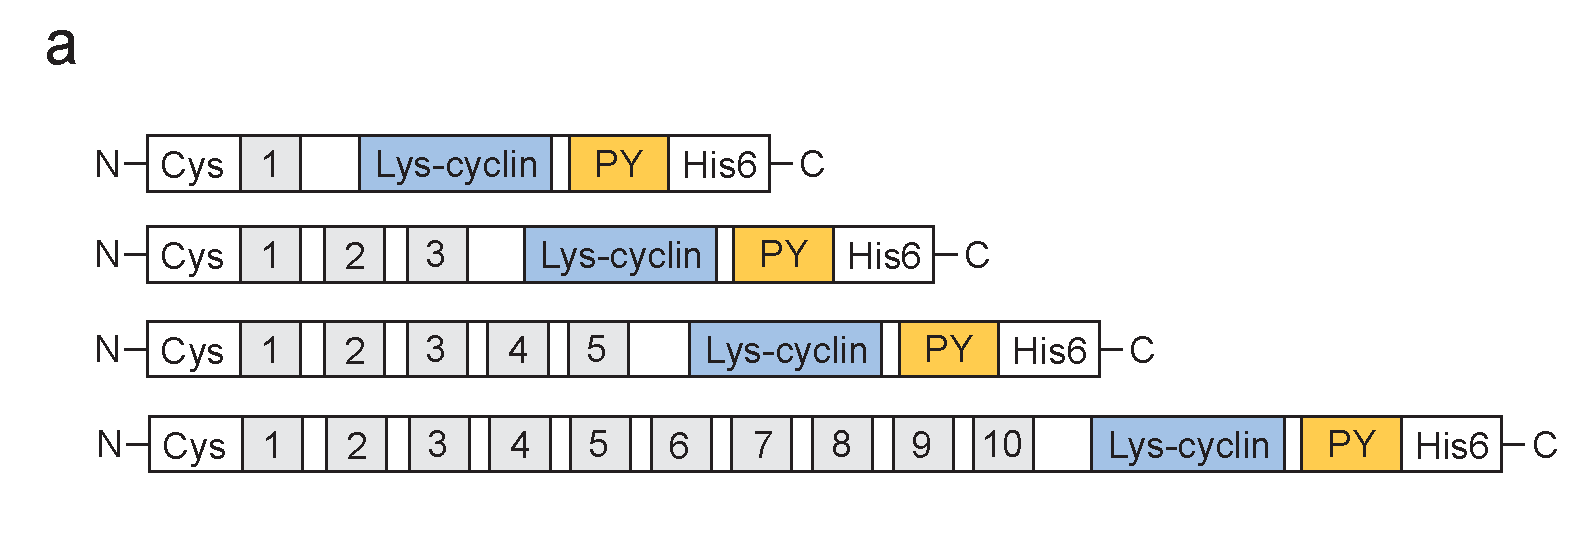
\includegraphics[scale=0.45]{titinconstructs}
	\label{fig:titinconstructs}}
\quad	
\subfigure{%
	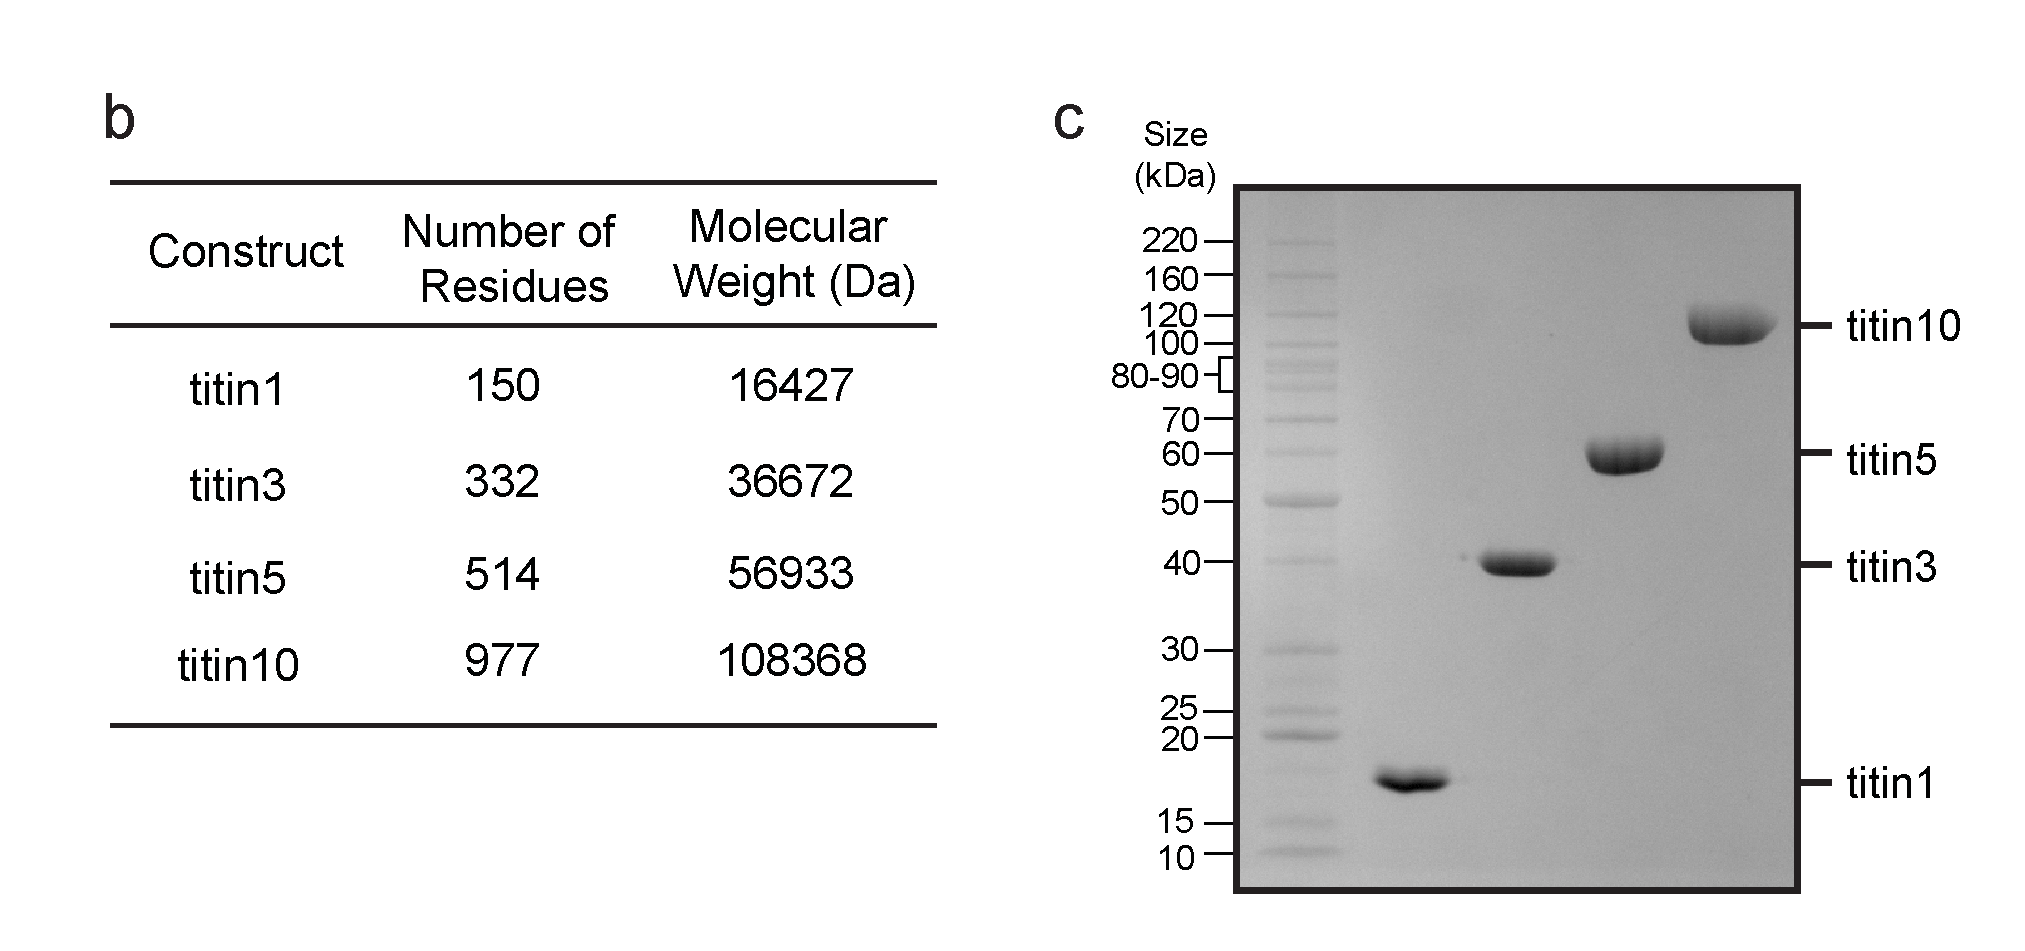
\includegraphics[scale=0.45]{titintablegel}
	\label{fig:titintablegel}}
%
\caption[Design and expression of titin concatamers]{Design and expression of titin concatamers.\par
\textbf{(a)} Predicted molecular weight for titin constructs. \textbf{(b)} Some more words.  \textbf{(c)} Some more words.
}
\label{fig:titin}
\end{figure}
%%-------------------------

%%-------------------------
\begin{figure}[H]
\centering
\subfigure{%
	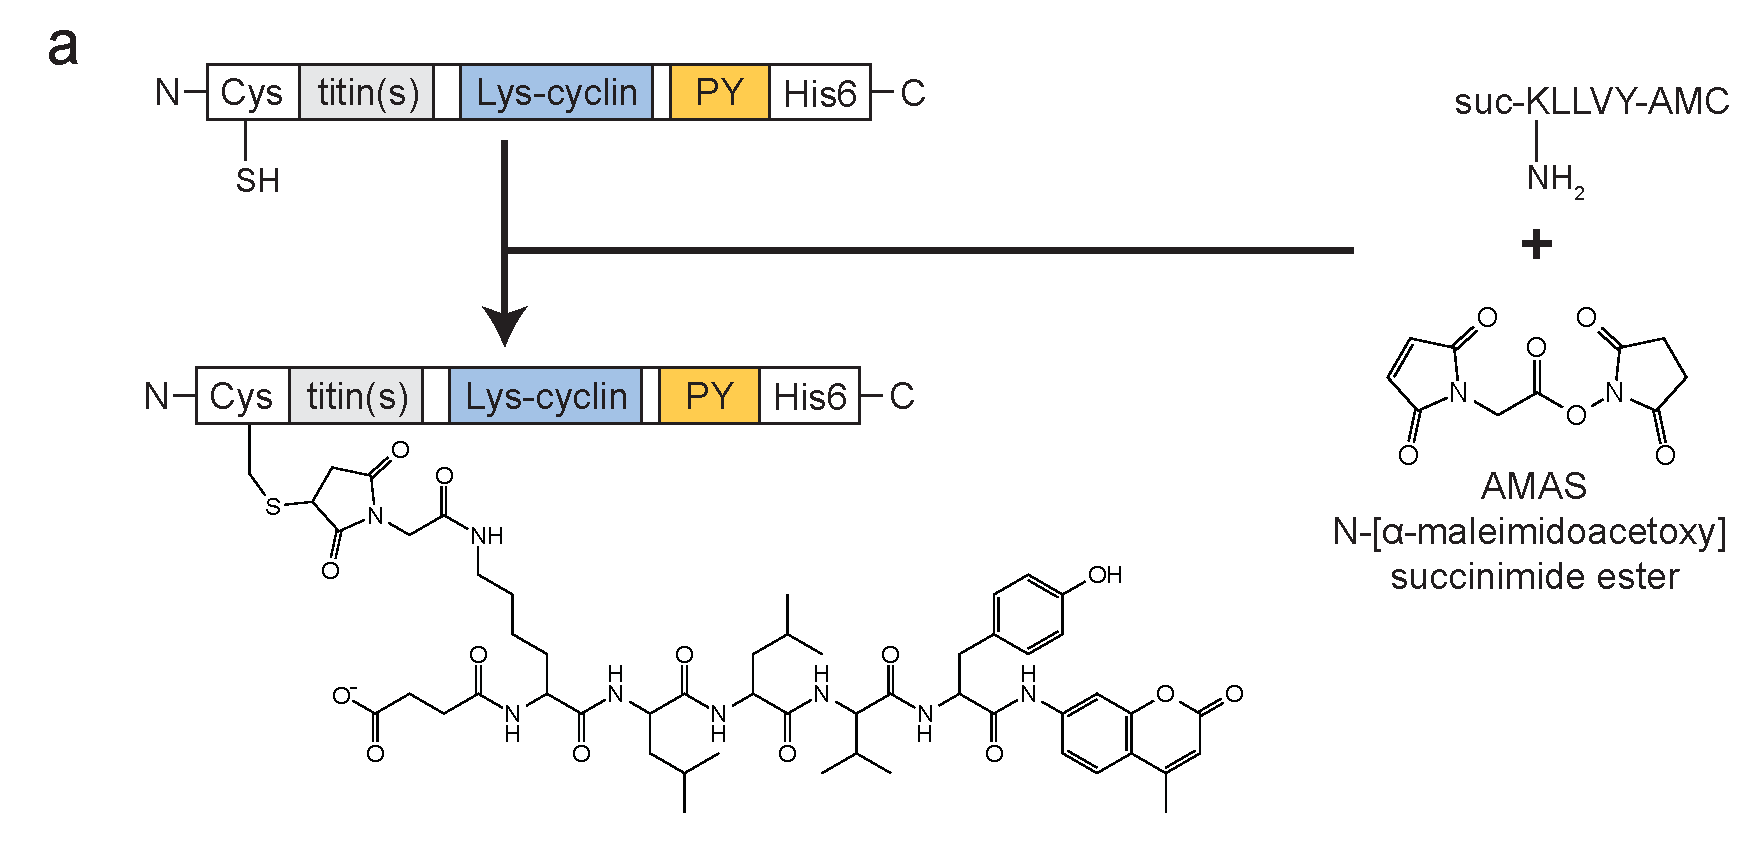
\includegraphics[scale=0.5]{titinstructure}
	\label{fig:titinstructure}}
\quad	
\subfigure{%
	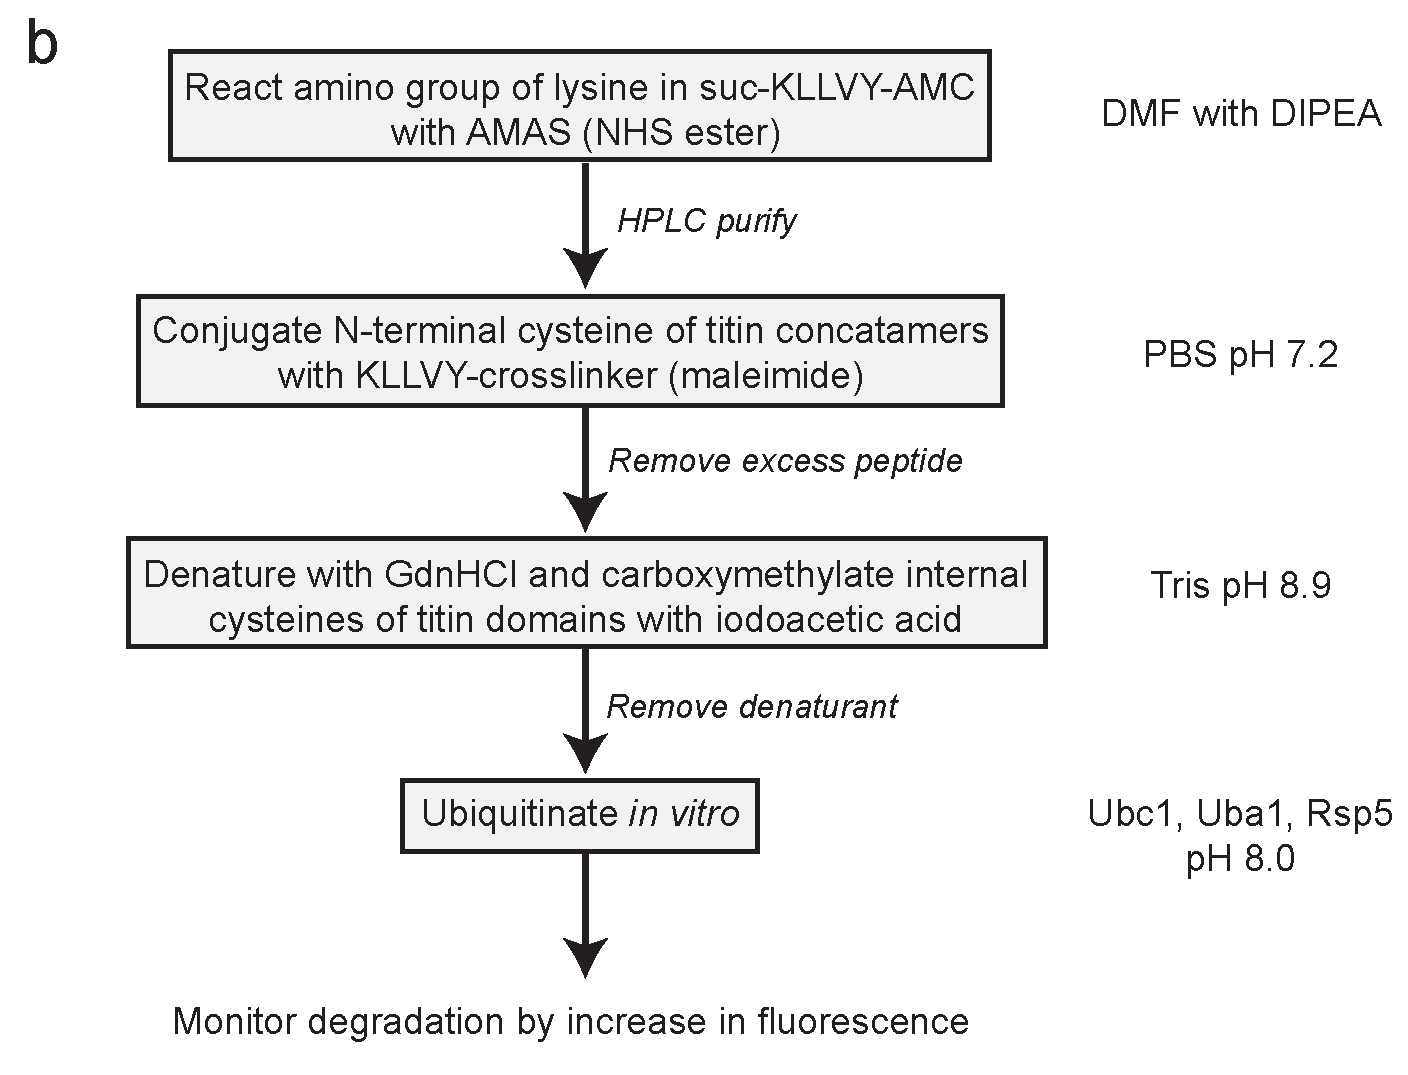
\includegraphics[scale=0.5]{reactionscheme}
	\label{fig:reactionscheme}}
%
\caption[title]{title.\par
\textbf{(a)} Predicted molecular weight for titin constructs. \textbf{(b)} Some more words.
}
\label{fig:titin}
\end{figure}
%%-------------------------

%%-------------------------
\begin{figure}[H]
\centering
\setlength{\fboxrule}{0pt}
\fbox{%
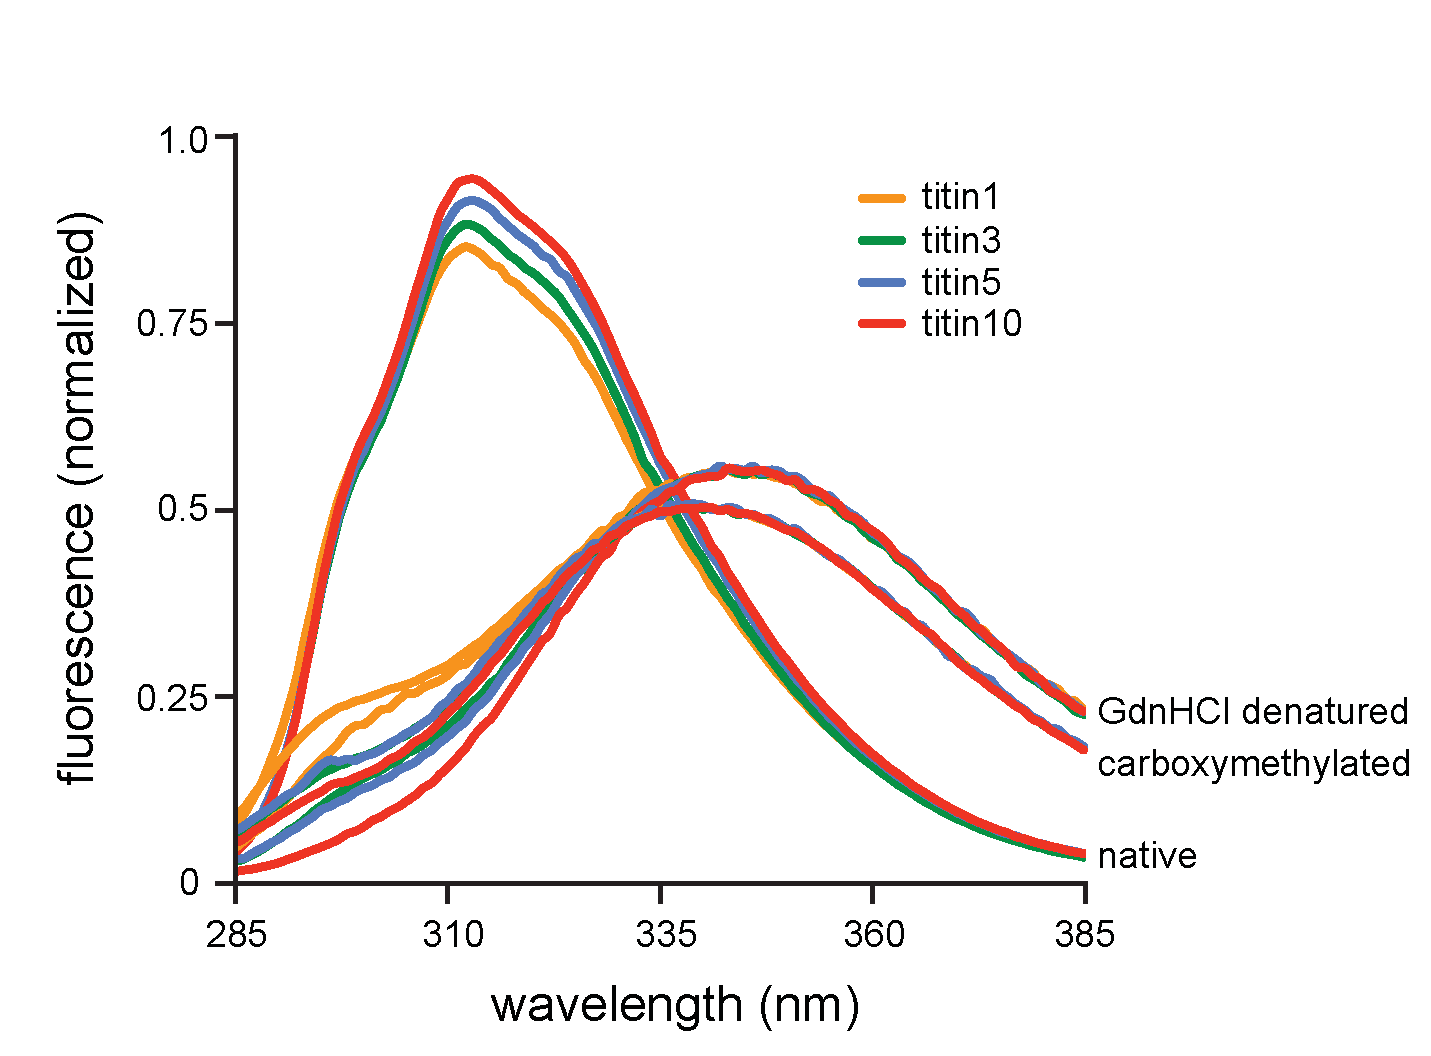
\includegraphics[width=0.9\textwidth]{trpfluor}%
}
\caption[Carboxymethylation of titin concatamers]{Carboxymethylation of titin concatamers.\par

}
\label{fig:titincarboxy}
\end{figure}
%%-------------------------




\subsection{Involvement of the arginine finger in subunit communication}
%table
	%RA, RK, EQRA?
%fig degradation bar graph



%%-------------------------

\section{Discussion}

%%-------------------------

\section{Materials and Methods}

\subsection{Cloning, expression and purification of titin concatemers}

\subsection{Labeling, carboxymethylation and ubiquitination of titin concatemers}

\subsection{Single and multiple turnover titin degradation assay}
%curve fits


%%-------------------------




\bibliography{library_robyn}{}

\appendix


% Appendix A

\chapter{October 2013 \textit{NSMB} Journal Cover}
\label{AppendixA}
\lhead{Appendix A. \emph{October 2013 \textit{NSMB} Journal Cover}}

\begin{figure}[h]
\centering
\setlength{\fboxrule}{1pt}
\fbox{%
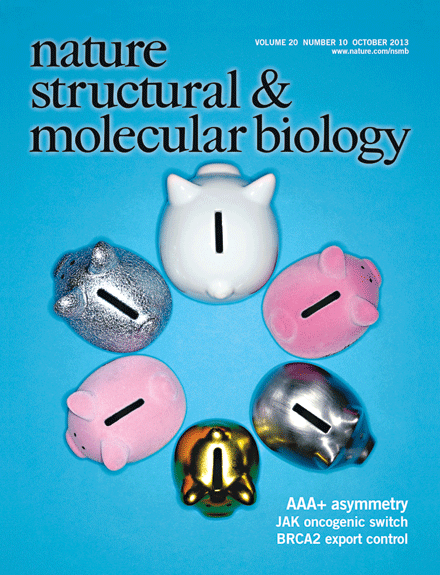
\includegraphics[scale=0.45]{cover}%
}
\caption[October 2013 Cover of \emph{NSMB}]{Cover of October 2013 Issue of \emph{Nature Structural \& Molecular Biology}.\par
The heterohexameric AAA+ complex of the eukaryotic 26S proteasome unfolds substrates prior to degradation. Martin and colleagues reconstitute proteasomes with recombinant subunits of the yeast unfoldase (Rpt1\---6) to reveal distinct roles of each. \copyright ~Andrew Paterson. pp 1164\---1172}
\label{cover}
\end{figure}




	

\chapter{Base Purification Protocol}
\label{AppendixB}
\lhead{Appendix B. Base Purification Protocol}

\textbf{OBJECTIVE}: Purification of base subcomplex from E. coli
\begin{itemize}
  \item Grow, induce and harvest liter\--scale cultures
  \item Nickel affinity column
  \item Anti\--FLAG affinity column
  \item Superose 6 gel filtration chromatography
\end{itemize}

%\vspace{0.75cm}
%\noindent\makebox[\linewidth]{\rule{\textwidth}{0.5pt}} 


\vspace{0.5cm}
\textbf{Purification buffers}\par
\textit{Make buffers without ATP/DTT, then add to the required amount of buffer prior to use}
\vspace{0.25cm}

\textbf{Nickel A}\par
25 mM HEPES, pH 7.6\par
100 mM NaCl\par
100 mM KCl\par
10\% glycerol\par
10 mM MgCl2\par
0.5 mM EDTA\par
20 mM imidazole\par
0.5 mM ATP\\

\textbf{Nickel B} \par
add 250 mM imidazole (solid) and re-adjust buffer to pH 7.6\\

\textbf{Gel filtration}\par
60 mM HEPES, pH 7.6\par
50 mM NaCl\par
50 mM KCl\par
10\% glycerol\par
5 mM MgCl2\par
0.5 mM EDTA\par
0.5 mM ATP\par
1 mM DTT\\


\textbf{Day 1}
\begin{itemize}
  \item Inoculate 50mL starter culture from cell stock
	\begin{itemize}
		\item Amp$^{res}:$ pETDUET (Rpn1/Rpn2/Rpn13)
		\item Kan$^{res}$: pCOLA (Flag-Rpt1/Rpt2/His-Rpt3/Rpt5/Rpt6/Rpt4)
		\item Chl$^{res}$: pACYC (chaperones Nas2/Nas6/Hsm3/Rpn14)
	\end{itemize}
  \item Grow overnight at 30�C\\
\end{itemize}


\textbf{Day 2}
\begin{itemize}
  \item Wash culture with dYT and inoculate each 1 liter flask with approximately 5mL of saturated overnight culture
  \item Grow large cultures at 37�C until OD$_{600}$ $=$ 0.4\--0.5 (2\--4 hours)
  \item Cool cultures to 18�C and induce at OD$_{600}$ $=$ 0.6\--0.8 with 1 mM IPTG overnight\\
\end{itemize}


\textbf{Day 3}
\begin{itemize}
  \item Harvest liter cultures by centrifuging at 4000 rpm for 20\--30 minutes
  \item Resuspend pelleted cells in 10 mL nickel A buffer per liter of culture
  \item Add lysozyme, benzonase and protease inhibitors (PMSF, leupeptin, aprotinin, pepstatin)
  \item Freeze at \--80�C\\
\end{itemize}


\textbf{Day 3-4}
\begin{itemize}
  \item Freeze-thaw cell lysates 2\--3 times total by thawing frozen lysate in cool or room temperature water and re\--freezing at \--80�C for at least a few hours\\
\end{itemize}


\textbf{Day 4}
\begin{itemize}
  \item Thaw frozen lysate
  \item Sonicate lysate in plastic container on ice: 90 \% power for 15 seconds on, 1 minute 30 seconds off for total sonication time of 1 minute 30 seconds
  \item Centrifuge lysate at 15,000 rpm for 30 minutes at 4C
  \item Wash nickel resin (50 \% slurry) twice with 25 ml nickel A buffer (use approximately 2 mL slurry per liter of culture)
  \item Incubate supernant with nickel resin for 30 minutes to 1 hour\\
  	\textit{All buffers from here on contain 0.5 mM ATP}
  \item Batch wash with nickel A buffer twice, then transfer resin to a column and wash until slow through no longer reacts with Bradford reagent.
  \item Elute with nickel B buffer in 1 mL aliquots
  \item Run pooled nickel eluate over a column containing 3-5 mL anti-FLAG M2 resin, repeat 3\--5 times
  \item Wash with 25\--50mL of nickel A buffer until flow through is clean
  \item Elute from FLAG column with nickel A buffer containing 0.15 mg ml$_{\--1}$ 3X FLAG peptide in 0.5 mL fractions
  \item Pool FLAG elute and add 5 mM DTT.  Concentrate volume to less than 500 $\mu$L using a 30,0000\-- or 100,000\--MWCO concentrator pre\--equilibrated with nickel A buffer
  \item Filter concentrated eluate through a small spin filter before performing gel filtration chromatography
  \item Run Superose 6 sizing column with gel filtration buffer containing 1 mM DTT and 0.5 mM ATP \\
\end{itemize}

	


% Appendix A

\chapter{List of constructs}
\label{AppendixC}
\lhead{Appendix C. List of base constructs}





	





\end{document}